% Options for packages loaded elsewhere
% Options for packages loaded elsewhere
\PassOptionsToPackage{unicode}{hyperref}
\PassOptionsToPackage{hyphens}{url}
\PassOptionsToPackage{dvipsnames,svgnames,x11names}{xcolor}
%
\documentclass[
  sn-nature,
]{sn-jnl}


\usepackage{xcolor}
\usepackage{amsmath,amssymb}
\setcounter{secnumdepth}{-\maxdimen} % remove section numbering
\usepackage{iftex}
\ifPDFTeX
  \usepackage[T1]{fontenc}
  \usepackage[utf8]{inputenc}
  \usepackage{textcomp} % provide euro and other symbols
\else % if luatex or xetex
  \usepackage{unicode-math} % this also loads fontspec
  \defaultfontfeatures{Scale=MatchLowercase}
  \defaultfontfeatures[\rmfamily]{Ligatures=TeX,Scale=1}
\fi
\usepackage{lmodern}
\ifPDFTeX\else
  % xetex/luatex font selection
\fi
% Use upquote if available, for straight quotes in verbatim environments
\IfFileExists{upquote.sty}{\usepackage{upquote}}{}
\IfFileExists{microtype.sty}{% use microtype if available
  \usepackage[]{microtype}
  \UseMicrotypeSet[protrusion]{basicmath} % disable protrusion for tt fonts
}{}
\makeatletter
\@ifundefined{KOMAClassName}{% if non-KOMA class
  \IfFileExists{parskip.sty}{%
    \usepackage{parskip}
  }{% else
    \setlength{\parindent}{0pt}
    \setlength{\parskip}{6pt plus 2pt minus 1pt}}
}{% if KOMA class
  \KOMAoptions{parskip=half}}
\makeatother
% Make \paragraph and \subparagraph free-standing
\makeatletter
\ifx\paragraph\undefined\else
  \let\oldparagraph\paragraph
  \renewcommand{\paragraph}{
    \@ifstar
      \xxxParagraphStar
      \xxxParagraphNoStar
  }
  \newcommand{\xxxParagraphStar}[1]{\oldparagraph*{#1}\mbox{}}
  \newcommand{\xxxParagraphNoStar}[1]{\oldparagraph{#1}\mbox{}}
\fi
\ifx\subparagraph\undefined\else
  \let\oldsubparagraph\subparagraph
  \renewcommand{\subparagraph}{
    \@ifstar
      \xxxSubParagraphStar
      \xxxSubParagraphNoStar
  }
  \newcommand{\xxxSubParagraphStar}[1]{\oldsubparagraph*{#1}\mbox{}}
  \newcommand{\xxxSubParagraphNoStar}[1]{\oldsubparagraph{#1}\mbox{}}
\fi
\makeatother

\usepackage{color}
\usepackage{fancyvrb}
\newcommand{\VerbBar}{|}
\newcommand{\VERB}{\Verb[commandchars=\\\{\}]}
\DefineVerbatimEnvironment{Highlighting}{Verbatim}{commandchars=\\\{\}}
% Add ',fontsize=\small' for more characters per line
\usepackage{framed}
\definecolor{shadecolor}{RGB}{241,243,245}
\newenvironment{Shaded}{\begin{snugshade}}{\end{snugshade}}
\newcommand{\AlertTok}[1]{\textcolor[rgb]{0.68,0.00,0.00}{#1}}
\newcommand{\AnnotationTok}[1]{\textcolor[rgb]{0.37,0.37,0.37}{#1}}
\newcommand{\AttributeTok}[1]{\textcolor[rgb]{0.40,0.45,0.13}{#1}}
\newcommand{\BaseNTok}[1]{\textcolor[rgb]{0.68,0.00,0.00}{#1}}
\newcommand{\BuiltInTok}[1]{\textcolor[rgb]{0.00,0.23,0.31}{#1}}
\newcommand{\CharTok}[1]{\textcolor[rgb]{0.13,0.47,0.30}{#1}}
\newcommand{\CommentTok}[1]{\textcolor[rgb]{0.37,0.37,0.37}{#1}}
\newcommand{\CommentVarTok}[1]{\textcolor[rgb]{0.37,0.37,0.37}{\textit{#1}}}
\newcommand{\ConstantTok}[1]{\textcolor[rgb]{0.56,0.35,0.01}{#1}}
\newcommand{\ControlFlowTok}[1]{\textcolor[rgb]{0.00,0.23,0.31}{\textbf{#1}}}
\newcommand{\DataTypeTok}[1]{\textcolor[rgb]{0.68,0.00,0.00}{#1}}
\newcommand{\DecValTok}[1]{\textcolor[rgb]{0.68,0.00,0.00}{#1}}
\newcommand{\DocumentationTok}[1]{\textcolor[rgb]{0.37,0.37,0.37}{\textit{#1}}}
\newcommand{\ErrorTok}[1]{\textcolor[rgb]{0.68,0.00,0.00}{#1}}
\newcommand{\ExtensionTok}[1]{\textcolor[rgb]{0.00,0.23,0.31}{#1}}
\newcommand{\FloatTok}[1]{\textcolor[rgb]{0.68,0.00,0.00}{#1}}
\newcommand{\FunctionTok}[1]{\textcolor[rgb]{0.28,0.35,0.67}{#1}}
\newcommand{\ImportTok}[1]{\textcolor[rgb]{0.00,0.46,0.62}{#1}}
\newcommand{\InformationTok}[1]{\textcolor[rgb]{0.37,0.37,0.37}{#1}}
\newcommand{\KeywordTok}[1]{\textcolor[rgb]{0.00,0.23,0.31}{\textbf{#1}}}
\newcommand{\NormalTok}[1]{\textcolor[rgb]{0.00,0.23,0.31}{#1}}
\newcommand{\OperatorTok}[1]{\textcolor[rgb]{0.37,0.37,0.37}{#1}}
\newcommand{\OtherTok}[1]{\textcolor[rgb]{0.00,0.23,0.31}{#1}}
\newcommand{\PreprocessorTok}[1]{\textcolor[rgb]{0.68,0.00,0.00}{#1}}
\newcommand{\RegionMarkerTok}[1]{\textcolor[rgb]{0.00,0.23,0.31}{#1}}
\newcommand{\SpecialCharTok}[1]{\textcolor[rgb]{0.37,0.37,0.37}{#1}}
\newcommand{\SpecialStringTok}[1]{\textcolor[rgb]{0.13,0.47,0.30}{#1}}
\newcommand{\StringTok}[1]{\textcolor[rgb]{0.13,0.47,0.30}{#1}}
\newcommand{\VariableTok}[1]{\textcolor[rgb]{0.07,0.07,0.07}{#1}}
\newcommand{\VerbatimStringTok}[1]{\textcolor[rgb]{0.13,0.47,0.30}{#1}}
\newcommand{\WarningTok}[1]{\textcolor[rgb]{0.37,0.37,0.37}{\textit{#1}}}

\usepackage{longtable,booktabs,array}
\usepackage{calc} % for calculating minipage widths
% Correct order of tables after \paragraph or \subparagraph
\usepackage{etoolbox}
\makeatletter
\patchcmd\longtable{\par}{\if@noskipsec\mbox{}\fi\par}{}{}
\makeatother
% Allow footnotes in longtable head/foot
\IfFileExists{footnotehyper.sty}{\usepackage{footnotehyper}}{\usepackage{footnote}}
\makesavenoteenv{longtable}
\usepackage{graphicx}
\makeatletter
\newsavebox\pandoc@box
\newcommand*\pandocbounded[1]{% scales image to fit in text height/width
  \sbox\pandoc@box{#1}%
  \Gscale@div\@tempa{\textheight}{\dimexpr\ht\pandoc@box+\dp\pandoc@box\relax}%
  \Gscale@div\@tempb{\linewidth}{\wd\pandoc@box}%
  \ifdim\@tempb\p@<\@tempa\p@\let\@tempa\@tempb\fi% select the smaller of both
  \ifdim\@tempa\p@<\p@\scalebox{\@tempa}{\usebox\pandoc@box}%
  \else\usebox{\pandoc@box}%
  \fi%
}
% Set default figure placement to htbp
\def\fps@figure{htbp}
\makeatother

\ifLuaTeX
  \usepackage{luacolor}
  \usepackage[soul]{lua-ul}
\else
  \usepackage{soul}
\fi

% definitions for citeproc citations
\NewDocumentCommand\citeproctext{}{}
\NewDocumentCommand\citeproc{mm}{%
  \begingroup\def\citeproctext{#2}\cite{#1}\endgroup}
\makeatletter
 % allow citations to break across lines
 \let\@cite@ofmt\@firstofone
 % avoid brackets around text for \cite:
 \def\@biblabel#1{}
 \def\@cite#1#2{{#1\if@tempswa , #2\fi}}
\makeatother
\newlength{\cslhangindent}
\setlength{\cslhangindent}{1.5em}
\newlength{\csllabelwidth}
\setlength{\csllabelwidth}{3em}
\newenvironment{CSLReferences}[2] % #1 hanging-indent, #2 entry-spacing
 {\begin{list}{}{%
  \setlength{\itemindent}{0pt}
  \setlength{\leftmargin}{0pt}
  \setlength{\parsep}{0pt}
  % turn on hanging indent if param 1 is 1
  \ifodd #1
   \setlength{\leftmargin}{\cslhangindent}
   \setlength{\itemindent}{-1\cslhangindent}
  \fi
  % set entry spacing
  \setlength{\itemsep}{#2\baselineskip}}}
 {\end{list}}
\usepackage{calc}
\newcommand{\CSLBlock}[1]{\hfill\break\parbox[t]{\linewidth}{\strut\ignorespaces#1\strut}}
\newcommand{\CSLLeftMargin}[1]{\parbox[t]{\csllabelwidth}{\strut#1\strut}}
\newcommand{\CSLRightInline}[1]{\parbox[t]{\linewidth - \csllabelwidth}{\strut#1\strut}}
\newcommand{\CSLIndent}[1]{\hspace{\cslhangindent}#1}



\setlength{\emergencystretch}{3em} % prevent overfull lines

\providecommand{\tightlist}{%
  \setlength{\itemsep}{0pt}\setlength{\parskip}{0pt}}





%%%% Standard Packages

\usepackage{graphicx}%
\usepackage{multirow}%
\usepackage{amsmath,amssymb,amsfonts}%
\usepackage{amsthm}%
\usepackage{mathrsfs}%
\usepackage[title]{appendix}%
\usepackage{xcolor}%
\usepackage{textcomp}%
\usepackage{manyfoot}%
\usepackage{booktabs}%
\usepackage{algorithm}%
\usepackage{algorithmicx}%
\usepackage{algpseudocode}%
\usepackage{listings}%

%%%%

\raggedbottom
\makeatletter
\@ifpackageloaded{caption}{}{\usepackage{caption}}
\AtBeginDocument{%
\ifdefined\contentsname
  \renewcommand*\contentsname{Table of contents}
\else
  \newcommand\contentsname{Table of contents}
\fi
\ifdefined\listfigurename
  \renewcommand*\listfigurename{List of Figures}
\else
  \newcommand\listfigurename{List of Figures}
\fi
\ifdefined\listtablename
  \renewcommand*\listtablename{List of Tables}
\else
  \newcommand\listtablename{List of Tables}
\fi
\ifdefined\figurename
  \renewcommand*\figurename{Figure}
\else
  \newcommand\figurename{Figure}
\fi
\ifdefined\tablename
  \renewcommand*\tablename{Table}
\else
  \newcommand\tablename{Table}
\fi
}
\@ifpackageloaded{float}{}{\usepackage{float}}
\floatstyle{ruled}
\@ifundefined{c@chapter}{\newfloat{codelisting}{h}{lop}}{\newfloat{codelisting}{h}{lop}[chapter]}
\floatname{codelisting}{Listing}
\newcommand*\listoflistings{\listof{codelisting}{List of Listings}}
\makeatother
\makeatletter
\makeatother
\makeatletter
\@ifpackageloaded{caption}{}{\usepackage{caption}}
\@ifpackageloaded{subcaption}{}{\usepackage{subcaption}}
\makeatother
\usepackage{bookmark}
\IfFileExists{xurl.sty}{\usepackage{xurl}}{} % add URL line breaks if available
\urlstyle{same}
\hypersetup{
  pdftitle={Quantifying the evolution of cycling network performance: A XX-city panel data analysis using open data},
  pdfauthor={Rosa Félix; David Levinson},
  pdfkeywords={template, demo},
  colorlinks=true,
  linkcolor={blue},
  filecolor={Maroon},
  citecolor={Blue},
  urlcolor={Blue},
  pdfcreator={LaTeX via pandoc}}


\title[Quantifying the evolution of cycling network performance: A
XX-city panel data analysis using open data]{Quantifying the evolution
of cycling network performance: A XX-city panel data analysis using open
data}

% author setup
\author[1]{\fnm{Rosa} \sur{Félix}}\author*[2]{\fnm{David} \sur{Levinson}}\email{david.levinson@sydney.edu.au}
% affil setup
\affil[1]{\orgdiv{CERIS}, \orgname{Instituto Superior Técnico -
University of Lisbon}, \orgaddress{\street{Av Rovisco Pais
1}, \city{Lisbon}, \country{Portugal}}}
\affil[2]{\orgdiv{School of Civil Engineering}, \orgname{University of
Sydney}, \orgaddress{\street{NSW
2006}, \city{Sydney}, \country{Australia}}}

% abstract 

\abstract{Despite significant investments in cycling infrastructure,
planning approaches often lack systematic methods to assess or simulate
their potential impacts on trip performance, stress, and accessibility.
Consequently, the holistic performance of the cycling network remains
under-evaluated. This research addresses this gap by integrating
geospatial and accessibility analysis into a replicable framework for
evaluating cycling networks across various stages of development. Using
open data, including historical OpenStreetMap networks and the Global
Building Atlas (LoD1), a systematic methodology was developed to assess
longitudinal changes in stress, performance and accessibility across XX
cities over five distinct periods over the last decade (2016-2026). For
each city, 20,000 OD pairs were generated based on buildings to simulate
realistic travel patterns, creating a massive panel dataset. A
fixed-effects panel data model was employed to estimate the elasticities
between specific types of cycling infrastructure investments and trip
performance metrics at both the macro (city-wide) and micro (route)
levels, to quantify how incremental network improvements translate into
tangible cycling benefits. Results highlight potential behavioral
trade-offs between route circuity, safety, and travel time. Furthermore,
\ldots{}}

% keywords
\keywords{template,  demo}

\begin{document}
\maketitle


\section{Main}\label{main}

{[}See examples of articles in Nature Cities - they follow a very
different structure!{]}

Sustainable and low-carbon cities are key for addressing climate change,
air pollution, and urban congestion.

Previous research found safe, high-quality and efficient cycling
networks play a crucial role in uptake cycling levels (P. Cambra and
Moura 2020; Christ et al. 2023; Félix, Cambra, and Moura 2020; Félix,
Lovelace, and Moura 2022; Félix, Moura, and Clifton 2019; Schoner and
Levinson 2014). In recent decades, several urban centers invested in
cycling infrastructure (Félix, Cambra, and Moura 2020). During COVID-19,
cities introduced pop-up bike lanes, but their planning was often not
evidence-based. Consequently, the outcome is a highly fragmented cycling
network due to a lack of cohesive strategies or ad-hoc, stretch-specific
planning approaches (Moura, Magalhães, and Santos 2017), lacking
efficiency.

These approaches often overlook the broader network, resulting in
missing links that hinder seamless and safe cycling connectivity.
\textbf{These missing links act as huge barriers for potential cyclists}
(Félix, Moura, and Clifton 2019), while minor infrastructure additions,
when solved, could significantly strengthen networks (Fernandes et al.
2020), providing great potential for cycling leverage (Félix, Moura, and
Clifton 2025), and allowing cyclists to safely bicycle between more
origins and destinations. Many authorities lack experience in cycling
network planning (Lovelace et al. 2017), reinforcing the need for
decision-making support tools regarding investments in cycling
infrastructure, that account for practical implementation barriers such
as urban planning constraints and funding limitations.

European cities are committed to meeting sustainable transport targets,
and increasing active travel. The Portuguese National Cycling Strategy
targets a 10\% shift from car to bicycle trips by 2030, with others
aiming to double or triple existing cycling levels for Carbon Neutrality
by 2050. The Lisbon Metropolitan Area (LMA) Sustainable Urban Mobility
Plan (SUMP) sets a strategy aiming to ``reduce the missing links in the
mobility and transport system, within the overall vision of metropolitan
cohesion'', based on the assumption that ``bridging these identified
discontinuities will make it possible to have continuous networks that
will solve the system's accessibility and attractiveness problems''
(\emph{TML, 2024}).

How, then, to identify the investment priorities to meet these targets?
Planning the infrastructure needed to change mobility patterns requires
high-quality evidence and adequate methods.

Recent research on cycling network performance and accessibility focuses
on developing comprehensive indicators and methodologies. Studies
assessed bike accessibility to activities and opportunities under
different network quality criteria, and developed indicators to track
cycling infrastructure improvements over time (Humberto, Félix, and
Moura 2023; Schoner and Levinson 2014; Schön, Heinen, and Manum 2024;
Van Der Meer, Werner, and Loidl 2024; Weikl and Mayer 2023; Macedo,
Rodrigues, and Tavares 2017), and ensure equitable network performance
across different areas (Humberto, Félix, and Moura 2023; Pereira et al.
2021).

Additionally, data-driven quality assessment methodologies have been
proposed, incorporating multiple criteria such as coherence,
fragmentation, directness, centrality, circuity, comfort, and
attractiveness (P. J. Cambra, Gonçalves, and Moura 2019; Costa, Marques,
and Moura 2021; Giacomin and Levinson 2015; Schön, Heinen, and Manum
2024; Van Der Meer, Werner, and Loidl 2024; Weikl and Mayer 2023; Werner
et al. 2024; Matos et al. 2021), yet \textbf{the definition of
``consistent'' / ``cohesive'' networks remains poorly defined}. Network
connectivity over spatial metrics is particularly relevant, yet
\textbf{more empirical evidence is needed to validate their effects on
cycling behavior} (Schoner and Levinson 2014; Schön, Heinen, and Manum
2024).

Nevertheless, few studies assessed its real impacts on cycling levels,
\st{which remains a gap in current research}. Tera, Hadachi, and
Pourmoradnasseri (2025) assesses the trip performance of new cycling
infrastructure in Tarfu (Estonia), using GPS data from the bike sharing
system, and measuring the improvements in terms of
\emph{\textbf{C}ompliance \textbf{R}atio} (``ratio of affected trips
among the trips that would utilize one of the study sites if the
time-optimal path was selected'') and \emph{\textbf{D}eviation
\textbf{R}atio} (tendency to detour for the sake of better
infrastructure, or ``the share of trips between OD-pairs whose shortest
path does not utilize any of the study sites among affected trips''),
and the \emph{\textbf{U}tilization \textbf{P}ercentage} (volume of trips
on those sites before and after the new bike facility)\emph{.}

Models and tools exist for cycling network prioritization (Félix,
Lovelace, and Moura 2022; Lovelace et al. 2017; Lovelace et al. 2024),
\textbf{but ignore network performance assessment}, despite using widely
available data in a city and open-source algorithms for reproducibility.
While computational limitations are less of an issue, transport
modeling, GIS, and graph science can be applied to \textbf{identify
missing links on given cycling networks with the potential to improve
network performance, accessibility, and cycling uptake}. These
approaches aim to provide planners with decision-making support tools to
evaluate existing networks, identify gaps and areas for improvement, and
prioritize infrastructure interventions.

Previous work identified missing links, using a proximity threshold
between fragmented groups of networks (Humberto, Félix, and Moura 2023).
This was done with the aim of identification, although no assessment was
made regarding the performance increase.

{[}Accessibility{]} Work from Rafael Pereira, Vale and Pereira (2016),
and Murphy and Owen (2019)

{[}Safety{]} Routing algorithms have different ways of weighting for a
``safer'' cycling route, in terms of objective safety. CycleStreets
consider infrastructure presence and type, traffic speed limits, volume
proxies (road hierarchy) and intersections. A most straight forward
measure was developed in Minesota, the Level of Traffic Stress (LTS),
and is being largely used (references). Concerns for the application in
different contexts, with different levels of cycling network development
and quality\ldots{}

This research addresses the following question: \textbf{What are the
cycling network trip performance, accessibility, and safety gains after
the expansion of a network?}

This research aims to assess the performance gains of networks, by
comparing the existing cycling networks with previous existing ones (3
year difference), and cumulative scenarios of adding (ranked) missing
links. The performance is assessed by:

\begin{itemize}
\item
  changes in trip distance (\emph{trip performance})
\item
  changes in circuity / deviation ratio (\emph{trip performance})
\item
  change in accessibility to opportunities (schools?)
  (\emph{accessibility})
\item
  changes the percentage of trip distance made in LTS1 and LTS2
  (\emph{safety})
\end{itemize}

The results show how the existing cycling network performance is
improved, by comparing with previous network, and with a network
expansion scenario of a missing-link provision intervention policy.
Results are then validated with count data (?) - although ``Existing
cycling behaviour and proximity to the bicycle path were associated with
the use of the new bicycle path. Increased use of the new bicycle path
as reported by the participants in the intervention area and increased
cycling recorded by the bike counts may be due to existing cyclists
changing routes to use the new path, and more cyclists from outside the
study area using the new path, as study participants did not increase
their frequency of cycling.'' (Rissel et al. 2015).

The cycling network new segments with higher gains are assessed and
discussed regarding their ``profile''/type (extension, connectivity
(degree, centrality measures).

The case study for application is Lisbon and Sydney (?), although the
methods can be applied to other cities, once we use open data
(OpenStreetMap) and tools.

{[}what is the novelty?{]}

The results support th decision policy of future interventions, helping
to quantify them in these components, in a reproducible manner.

The motivation for this research stems from the need to systematically
address these gaps, offering cities a replicable methodology and digital
tool to \st{identify and} assess and prioritize key network
improvements. The challenge lies in integrating emerging graph-based
programming techniques to model, simulate, and prioritize impactful
cycling connections. Bridging these gaps, cities enable safer, more
accessible networks that attract potential cyclists.

\section{Literature review - remove and incorporate in the
Background}\label{literature-review---remove-and-incorporate-in-the-background}

Namely for: performance indicators (network structure measures) as
predictors for bicycle commuting levels;

We started with Schoner and Levinson (2014): connectivity and directness
(network structure measures) as predictors for bicycle commuting levels.

\textbf{Coherent}: ``forming continuous networks linking origins and
destinations.'' (Wang et al. 2026).

The work from Niaki et al. (2025) was promising, once they assess
``Cycling \textbf{Discontinuities}'' as indicators for performance
evaluation. They apply the method to 4 cities: Montreal, Vancouver,
Portland, and Washington D.C. Very recent article, presented in WCTR
2023.

\begin{quote}
``Reviewing existing evaluation methods, it further appears that
connectivity or discontinuity indicators \textbf{have not been
systematically identified} and are missing from many evaluation
methods.''
\end{quote}

\begin{quote}
``proposes a set of indicators to measure cycling network connectivity
and the \textbf{methodology to calculate them}, including automated
methods for geospatial data with the
\href{https://github.com/nsaunier/cycling-discontinuities}{code
available} under an open-source licence'' (Uses SpatialLite, 8yrs old)
\end{quote}

But, in the end, the consideration of discontinues has a different
meaning from what we are looking for. They consider them as a
\textbf{change of cycling infrastructure type} and network endpoints.

From Schön, Heinen, and Manum (2024), they provide a literature review
on cycling network connectivity and its effects on cycling. They
categorize papers using network graph theories (betweenness, centrality,
etc); circuity; accessibility; angular segment analysis; LOS/LTS;
network growth algorithms and network design problems (NGA/NDP),
optimising cycling network coverage under cost constraints.

\begin{quote}
there is a trend towards more comprehensive and complex measures
focusing on l\textbf{ink prioritisation, cost-efficient gap closures},
travel demand or several connectivity aspects simultaneously. Such
measures allow more comprehensive studies of networks, but we emphasise
the importance of \textbf{open-source data, codes and software} to make
these recent and future measures and methodologies accessible to
practitioners and researchers.
\end{quote}

\begin{quote}
``no review has been dedicated to the measures, methods and models
applied to assess network connectivity or the \textbf{impact of
increased network connectivity} on cycling behaviour''

``The findings suggest an increase in the number of publications on
network connectivity up to 2019, followed by a plateau in the number of
studies but with \textbf{more complex methods}.''

``empirical verifications regarding the \textbf{effects of network
connectivity on travel behaviour} remain a research gap, even in
high-cycling countries, with evidence further limited by \textbf{limited
link-level travel data}''
\end{quote}

Network-based measures apply network analysis (Cooper 2015) which
considers the entire network available to cyclists, evaluating its
ability to connect specific origins and destinations or to connect
links/nodes to all other links/nodes in a network.

Network analysis can grasp the effects of missing links or links with
poor cycling infrastructure, which is particularly important for
inexperienced and young cyclists, as they tend to value the presence of
continuous cycling infrastructure more than experienced cyclists
(Bernhoft and Carstensen 2008; Heinen, Wee, and Maat 2010). Assessing
the connectivity of an entire network can be complex and computationally
demanding, and requires detailed and topologically correct network
models (Boeing 2017).

Vale and Pereira (2016) review of operational measures of walking and
cycling accessibility concluded that cycling \textbf{accessibility} had
received little attention and was a major field for future research.

The Cycling Routing Algorithm for Network Connectivity (CRANC) tool
(Gehrke et al. 2020) evaluates the benefits of new bicycle facilities
for the \textbf{accessibility} of various populations and
neighbourhoods. It integrates cyclist type/profile and LTS in route
choice. \textbf{This tool is not open, and we cannot use it.}

Reggiani et al. (2022) explores the detour acceptance and
``\textbf{discomfort}''. Bikeability curve with pareto frontier routes.

\begin{quote}
The relative distance, also referred to as \textbf{circuity} in the
remainder of the article, is the route distance (sum of all path links)
divided by the Euclidean distance. This measure, used also in Schoner
and Levinson (2014), allows identifying if there are OD pairs connected
by meandering routes, \textbf{which may suggest the need for new road
infrastructure}. The purpose of this measure is to ``identify
recreationally oriented routes that meander or circle back on
themselves, versus routes that provide an efficient utilitarian
connection for commuting'' as pointed out in Schoner and Levinson
(2014).

The \textbf{relative discomfort} is defined as the total discomfort of
the route (sum of discomfort on all links of the route) divided by the
Euclidean distance (in meters) of the shortest route. The resulting
relative discomfort represents the discomfort per meter.\\
It is related with the number of different facility types travelled, and
the distance traveled in a mix traffic environment.

There are many ways to combine the \textbf{Pareto fronts of all
different OD-pairs} into one single so-called network-wide bikeability
curve. An approach that transforms the set of Pareto fronts into
\textbf{one single network-wide bikeability curve}. This curve contains
for all possible distance-discomfort trade-off choices, the expected
distance, and discomfort of the optimal route for an OD-pair that is
sampled from an OD-demand distribution.
\end{quote}

(explore more the methods of this paper!)

Furth, Mekuria, and Nixon (2016) define ``lack of connectivity''
measured by the fraction of OD pairs which are connected with the use of
high LTS, excessive detours, weighted by travel demand.

\begin{quote}
When streets with high traffic stress - on which the mainstream
population is unwilling to ride a bike - are removed, the remaining
network of streets and paths can be fragmented and poorly connected.
\end{quote}

Schön, Heinen, and Manum (2026) assesses the impact of a new cycling
infrastructure segment (a bridge in Norway) in terms of betweenness and
route link density improvements, and estimate the increase in cycling
probabilities.

\pandocbounded{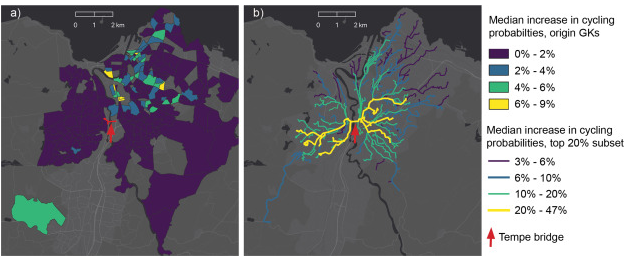
\includegraphics[keepaspectratio]{../images/clipboard-3285979495.png}}

A very recent paper from Wang et al. (2026) provides a framework for
generating and prioritizing ``core'' cycling network designs.

It tackles fragmented and disjointed networks. They balance cohesion
coverage and directness metrics, aimed to produce ``effective'' networks
for the cycling potential, meeting the travel patterns. The result are
``cohesive'' networks suggested, using an
\href{https://github.com/nptscot/corenet}{open-source tool} developed by
the authors. The process takes about 15min to run and generate results
(!).

\begin{quote}
While the method uses graph theory concepts for network analysis, it is
fundamentally driven by travel demand data and policy objectives
\textbf{rather than network structure alone}. It \textbf{does not
consider} \textbf{current cycling volumes}, but \textbf{cycling
potential estimates}.
\end{quote}

It considers the following criteria based on data availability and
computational feasibility: \textbf{directness} (through arterial
weighting and shortest-path algorithms), \textbf{connectivity and
coherence} (via network growth strategies and systematic removal of
disconnected segments), \textbf{coverage and accessibility} (through
spatial analysis and buffer zone evaluation), and \textbf{demand
alignment} (by integrating cycling potential data to focus on high-usage
corridors).

Hierarchical road prioritization and arterial weighing:

\begin{enumerate}
\def\labelenumi{\arabic{enumi}.}
\tightlist
\item
  Routes with higher cycling potential are prioritised.
\item
  When cycling potential is comparable, ``A Road'' segments are chosen
  over ``B Road'' segments, which in turn are chosen over ``Minor Road''
  segments.
\item
  When cycling potential values are identical, the network favours
  routes associated with higher-ranked road types.
\item
  If both cycling potential values and road classifications are
  equivalent, the shortest route is selected.
\end{enumerate}

Key performance metrics assess Network Cohesion and Connectivity, Demand
Alignment, Origin-Destination Accessibility, Directness and Efficiency.
(\emph{read more about the ones of interest})

\pandocbounded{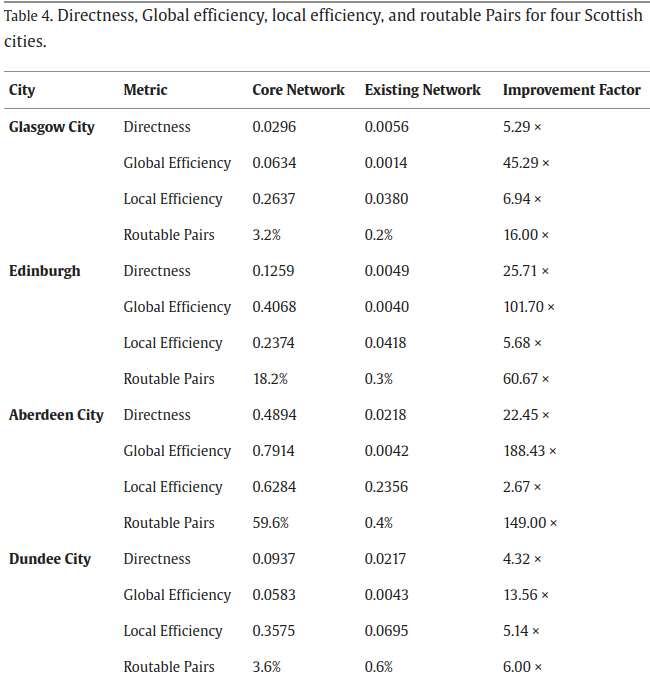
\includegraphics[keepaspectratio]{../images/clipboard-2027430881.png}}

It is well suited for places without cycling network, or to compare the
results with places with already implemented networks. They also discuss
the problems with raw OSM data (topological, miss-classification,
cycling and pedestrian as separated lines from the road network).

\subsection{Network structures and
topology}\label{network-structures-and-topology}

A lot of work has been developed using \textbf{synthetic} networks and
synthetic population / demand. -\textgreater{} We are using real world
data

For the generality of road network structures, the work from Xie and
Levinson (2007) analyze topology and geometric variations on 16 types of
(synthetic) networks. It is focused on the travel perspective.

From Xing et al. (2025), a definition of Road Network Connectivity is
established, which is binary (connected or unconnected), and does not
provide performance levels.

\begin{quote}
Graph theory was the earliest method used in the study of road network
connectivity evaluation
{[}\href{https://onlinelibrary.wiley.com/doi/full/10.1155/atr/3589423\#bib-0022}{22}{]}
and it is a feasible and effective method to study road network
connectivity as a complex topological network
{[}\href{https://onlinelibrary.wiley.com/doi/full/10.1155/atr/3589423\#bib-0023}{23}{]}.
Most of the definitions of road network connectivity in graph theory are
defined in terms of the topological connectivity relationship between
nodes, and if two neighboring nodes are linked by an edge, they are said
to be connected
{[}\href{https://onlinelibrary.wiley.com/doi/full/10.1155/atr/3589423\#bib-0024}{24}{]}.
In this context, the road network connectivity is defined from the
\textbf{graph theory level}, where the road network is treated as a
topological network, and the road network connectivity is evaluated
based on the topological relationships between nodes and edges.

However, it is difficult to fully express road network connectivity in
an increasingly \textbf{complex urban road network} only by defining
road network connectivity in a limited space from the perspective of
road network topology. This definition of road network connectivity only
through a simple topology can only distinguish between connectivity and
non-connectivity, and \textbf{cannot describe different degrees of
connectivity performance}.
\end{quote}

The traditional connectivity index was proposed in the 20th century,
when the road traffic structure and the urban road network were simpler
than today. Then they propose a road network connectivity evaluation
method based on node \textbf{turning coefficients} to address
connectivity challenges under complex traffic control conditions. And
run for different neighbourhoods, This is more from a traffic
perspective (turning lane turning restrictions).

Szell et al. (2021) examined topological constraints and strategic
planning for cycling network optimisation using \textbf{percolation}
theory. Their synthetic approach modelled cycling network growth in
\textbf{62 cities}, testing three growth strategies: random addition,
greedy demand-based expansion, and betweenness centrality
prioritisation. Their findings reveal challenges in creating
\textbf{cohesive networks} and demonstrate diminishing returns on
cycling infrastructure investment until reaching critical mass,
highlighting the need for strategic, persistent investment. Whilst their
network expansion models show significant overlaps with well-developed
cycling networks in cities, the synthetic approach using theoretical
node placement and uniform grid topologies does not directly represent
real urban street patterns or empirical demand distributions. (from Wang
et al. (2026) lit review). {[}\emph{explore this further}{]}

\subsection{Accessibility}\label{accessibility}

Check the work from Murphy and Owen (2019)

\subsection{So\ldots{}}\label{so}

\textbf{Consistency/cohesion} (working definition to test):

\begin{itemize}
\item
  continuous connections between origins/destinations
\item
  low-stress continuity along likely routes
\item
  minimal fragmentation/dangling segments
\item
  good directness + redundancy at a network level
\end{itemize}

Summary from the literature so far:

\begin{itemize}
\item
  Connectivity/discontinuity indicators: Niaki et al. (2025) (cycling
  discontinuities): useful methods + code, but their ``discontinuity''
  focuses on facility-type change/endpoints (not fully my target
  meaning)
\item
  Reviews: Schön, Heinen, and Manum (2024) on connectivity measures +
  limited empirical validation
\item
  Directness/circuity and discomfort: Schoner and Levinson (2014)
  (circuity), Reggiani et al. (2022) (distance--discomfort Pareto)
\item
  Network growth / critical mass: Szell et al. (2021) (percolation -
  needs further exploring)
\item
  ``Core/cohesive network'' generation: Wang et al. (2026) framework +
  open tool (but uses cycling potential, not observed volumes)
\end{itemize}

\begin{enumerate}
\def\labelenumi{\arabic{enumi}.}
\tightlist
\item
  How can ``consistent'' cycling networks be defined and
  operationalised?
\item
  How does increasing network consistency affect -\textgreater{}
  Accessibility -\textgreater{} cycling adoption/ridership?
\end{enumerate}

\section{Results}\label{results}

\subsection{Macro level: city-wide}\label{macro-level-city-wide}

\subsection{Micro level: routes}\label{micro-level-routes}

\section{Discussion}\label{discussion}

Impact estimation can be assessed with count data available for
different years (modelling the effects)

\subsection{The use of OpenStreetMap
data}\label{the-use-of-openstreetmap-data}

OpenStreetMap (OSM) datasets provide a common dataset for road networks
(including cycling infrastructure), available mostly worldwide. However,
OSM is a community-based and volunteer open dataset, which means that
the detail of information increases with time, but does not mean that
the road network was not always there in the real world. This can be
verified with the size of the extracted osm.pbf files from
\href{https://www.geofabrik.de/}{geofabrik} (the largest OSM
repository), for the different years (Table X) showing an increase in
amount of data available for each selected city region.

\begin{Shaded}
\begin{Highlighting}[]
\CommentTok{\# run this only in the server, where the pbf files live}

\CommentTok{\# library(dplyr)}
\CommentTok{\# library(stringr)}
\CommentTok{\# library(knitr)}
\CommentTok{\# }
\CommentTok{\# file\_list \textless{}{-} list.files(path = "../data/osm\_pbf/", full.names = TRUE)}
\CommentTok{\# \# file\_list}
\CommentTok{\# \# file\_list = file\_list}
\CommentTok{\# }
\CommentTok{\# file\_info \textless{}{-} file.info(file\_list)}
\CommentTok{\# }
\CommentTok{\# df \textless{}{-} data.frame(}
\CommentTok{\#   filename = basename(rownames(file\_info)),}
\CommentTok{\#   size\_mb = file\_info$size / (1024 * 1024) \# convert in MB,}
\CommentTok{\# )}
\CommentTok{\# }
\CommentTok{\# summary\_table \textless{}{-} df |\textgreater{} }
\CommentTok{\#   mutate(year = paste0("20", str\_extract(filename, "(?\textless{}={-})\textbackslash{}\textbackslash{}d\{2\}")))|\textgreater{} \# 4 digits year }
\CommentTok{\#   group\_by(year) |\textgreater{} }
\CommentTok{\#   summarise(}
\CommentTok{\#     mean\_size\_MB = mean(size\_mb, na.rm = TRUE),}
\CommentTok{\#     median\_size\_MB = median(size\_mb, na.rm = TRUE),}
\CommentTok{\#     total\_files = n()}
\CommentTok{\#   )}

\NormalTok{summary\_table }\OtherTok{=} \FunctionTok{read.csv}\NormalTok{(}\StringTok{"../data/osm\_file\_size\_summary.csv"}\NormalTok{)}

\FunctionTok{kable}\NormalTok{(summary\_table }\SpecialCharTok{|\textgreater{}} \FunctionTok{filter}\NormalTok{(year }\SpecialCharTok{!=} \StringTok{"20NA"}\NormalTok{) }\SpecialCharTok{|\textgreater{}} \FunctionTok{select}\NormalTok{(}\SpecialCharTok{{-}}\NormalTok{total\_files), }\CommentTok{\# there is one more irrelevant for now}
      \AttributeTok{digits =} \DecValTok{0}\NormalTok{, }
      \AttributeTok{col.names =} \FunctionTok{c}\NormalTok{(}\StringTok{"Year"}\NormalTok{, }\StringTok{"mean file size (MB)"}\NormalTok{, }\StringTok{"median file size (MB)"}\NormalTok{),}
      \AttributeTok{caption =} \StringTok{"Mean and Median OSM File Sizes by Year"}\NormalTok{)}
\end{Highlighting}
\end{Shaded}

OSM tagging is not consistent over years, which may lead to
inconsistency issues of the results, since we are using the same
classification of cycling infrastructure for the three year periods. For
instance, the classification for Munich (Germany) changes drastically
with time, and it does not mean that the infrastructure itself changed -
only the tags in OSM did.

\begin{figure}[H]

{\centering \pandocbounded{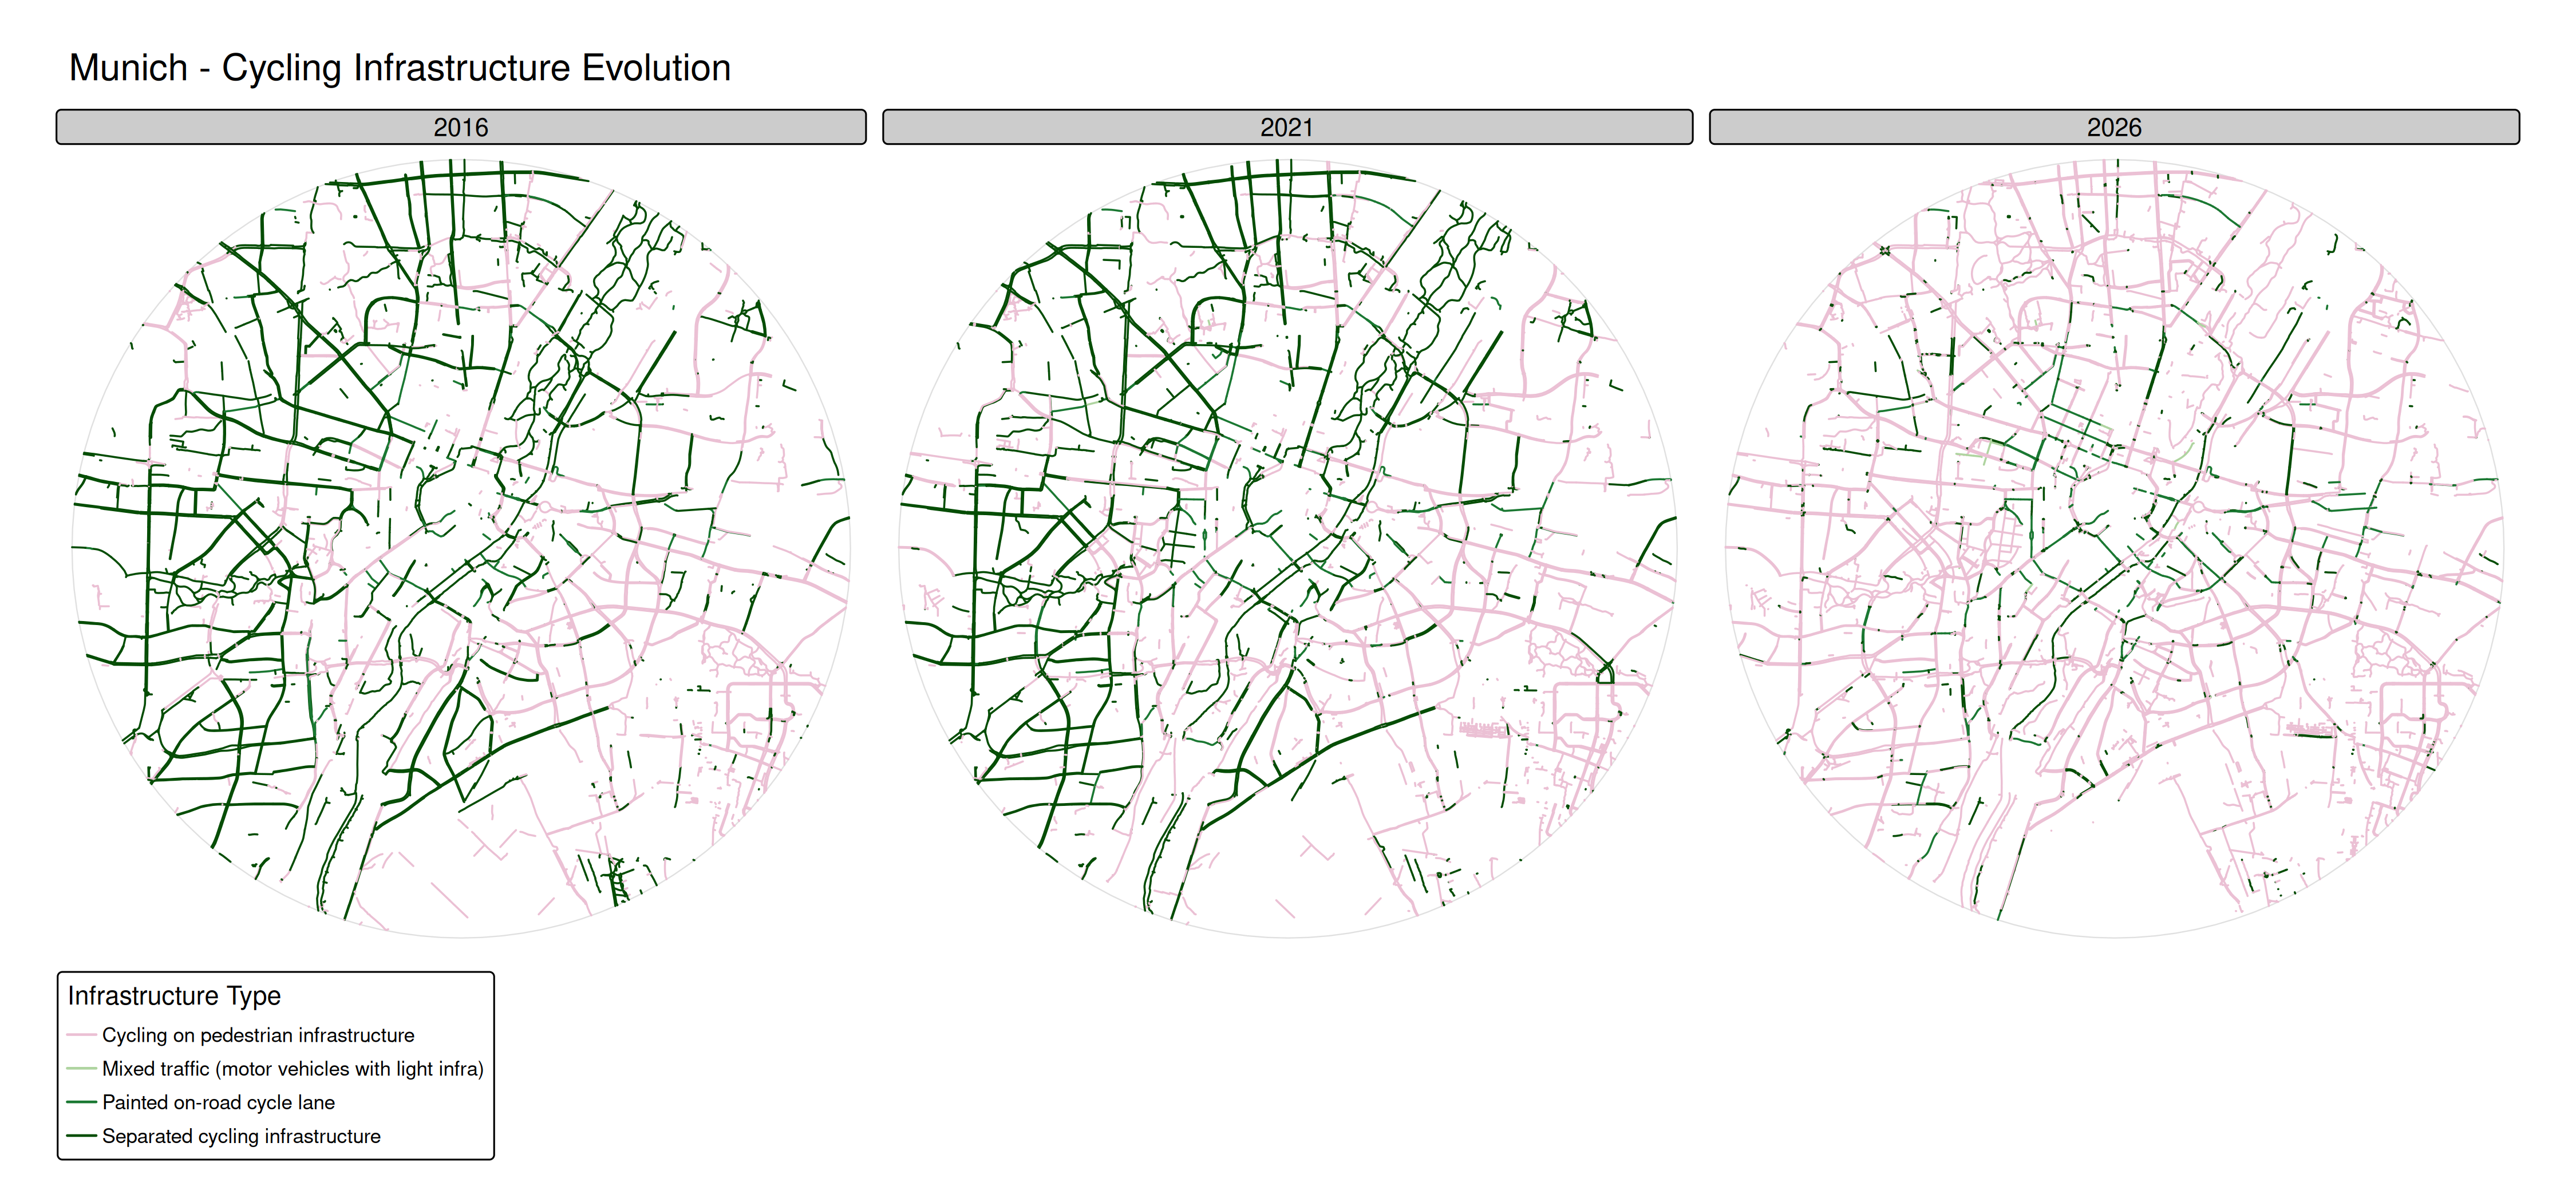
\includegraphics[keepaspectratio]{../data/pipeline/munich/results/ci_evolution_facet_map.png}}

}

\caption{Cycling infrastructre classification for Munich in 2016, 2021
and 2026. There is a massive change in segments' tagging between 2021
and 2026.}

\end{figure}%

Additionally tags can become deprecated and new tags can emerge. For
instance, in June 2025, the OSM community submitted a
\href{https://wiki.openstreetmap.org/wiki/Proposal:Deprecate_cycleway\%3Dopposite_family}{proposed
an voted} in favour for a new way of tagging cycling contra-flows that
do not have dedicated infrastructure - which are common in Paris or
Munich. Our custom reclassification of cycling infrastructure in fewer
types does not account for this. There are some attempts to directly
classify the safety of a cycling infrastructure segment in OSM, with
\texttt{class:bicycle=*} (values from -3 ``Avoid at all costs'', to 3
``This path is so beautiful, it's worth taking a detour''), but it is
\href{https://wiki.openstreetmap.org/wiki/Key:class:bicycle}{still under
dispute}.

\subsection{The use of LTS}\label{the-use-of-lts}

LTS does not account for the quality of the cycling infrastructure.

Routing engine also does not account for other variables, such as
gradients.

\section{Methods}\label{methods}

\textbf{State of the art and selection of network indicators}

\begin{itemize}
\item
  Literature review on cycling network analysis and performance
\item
  Systematization of network indicators with impact on cycling levels
\end{itemize}

A comprehensive set of network performance indicators will be compiled
from the literature and case-studies on cycling network assessment
regarding consistency, performance and accessibility. These indicators
include (not exclusively) connectivity, directness, closeness,
betweenness, redundancy, and fragmentation. The integration of open data
sources and graph network science will advance the field of cycling
network analysis.

\textbf{Modelling network factors with impact on cycling adoption}

Collecting and processing data to build a model that explains how
improvements in network consistency influence performance. This model is
calibrated and validated with the existing high-quality cyclists'
counting dataset in the case studies (2017-2023), coincident with the
before/after major cycling infrastructure changes in each city.

For \textbf{data preparation}

\begin{itemize}
\item
  OSMnx, for creating a valid topological network, with edges and nodes
  correctly represented. There is a QGIS plugin for that. See Boeing
  (2017) .
\item
\end{itemize}

For \textbf{identification of missing links}

\begin{enumerate}
\def\labelenumi{\arabic{enumi}.}
\tightlist
\item
  Network performance assessment (baseline)
\item
  Simulate changes in the cycling network (scenarios)
\item
  Assess performance of potential improvements and estimate impacts on
  cycling
\item
  Identify network segments and prioritize high-impact interventions
\item
  Develop an automated algorithm to systematically identify priority
  network links
\end{enumerate}

\begin{itemize}
\item
  \texttt{sfnetworks} R package
\item
  sDNA, from Cooper and Chiaradia (2020), although it is not easy to
  setup (only windows a couple of years ago), and very useful for 3D
  networks (as Hong Kong PedNet)
\end{itemize}

For the \textbf{impacts estimation}

\begin{itemize}
\tightlist
\item
  Modelling with panel data? considering the temporal effects (existing
  network at each year), and location and global effects
\end{itemize}

\subsection{Cities}\label{cities}

Cities, city centers coordinates from list, buffer of 10 km - to be more
comparable (and also many cities do not have limits well established
(can be districts, metropolitan areas, and so on)

Also, because some places do not have a good definition of ``city'' or
``metropolitan area'' as an administrative area (polygon).

List of +700 cities worldwide, with \textgreater{} 1 million residents,
lat and lon from the historical city center or CBD
(\url{https://gist.github.com/nkrusch/848e4d6ca0be879e2e03b78b051f17da})

List of +48k cities worldwide (World Cities Database\footnote{We're
  proud to offer a simple, accurate and up-to-date database of the
  world's cities and towns. We've built it from the ground up using
  authoritative sources such as the NGIA, US Geological Survey, US
  Census Bureau, and NASA.} -
\url{https://simplemaps.com/data/world-cities} )

List from People for Bikes with city ratings regarding a score of
cycling friendly cities, as 2025
(\url{https://cityratings.peopleforbikes.org/ratings})

The rationale to select the 50 cities was:

\begin{itemize}
\tightlist
\item
  Cities that faced some improvements in cycling infrastructure in the
  last 10 years, for instance during the pandemic
\item
  Cities with cycling data (checked against People4Bikes index scores
  for 2025)
\item
  Excluded cities with consolidated cycling network (that didn't change
  much) such as Amsterdam or Copenhagen - outliers
\item
  Widelly geographical distribution, equilibrium
\item
  A minimum of 20 km of cycling infrastructure in jan 2026: this
  excludes many sub-tropical cities.
\item
  A reasonable good OSM data quality and availability - this excludes
  most of China (remove?)
\item
  Internationally renown cities
\end{itemize}

Use a 10km projected buffer from city center, that defines the city
areas for this research, for comparison purposes

The 50 cities are as follows:

{[}table with city, country{]}

\begin{Shaded}
\begin{Highlighting}[]
\NormalTok{city\_list }\OtherTok{=} \FunctionTok{read.csv}\NormalTok{(}\StringTok{"../data/city\_list.txt"}\NormalTok{)}
\FunctionTok{names}\NormalTok{(city\_list) }\OtherTok{=} \FunctionTok{c}\NormalTok{(}\StringTok{"city"}\NormalTok{, }\StringTok{"lat"}\NormalTok{, }\StringTok{"lon"}\NormalTok{, }\StringTok{"population"}\NormalTok{, }\StringTok{"country"}\NormalTok{, }\StringTok{"countrycode"}\NormalTok{, }\StringTok{"building\_tile"}\NormalTok{)}
\NormalTok{selected\_cities }\OtherTok{=} \FunctionTok{c}\NormalTok{(}
    \StringTok{"Sydney"}\NormalTok{, }\StringTok{"Lisbon"}\NormalTok{, }\StringTok{"Paris"}\NormalTok{, }\StringTok{"Barcelona"}\NormalTok{,}
    \StringTok{"Munich"}\NormalTok{, }\StringTok{"London"}\NormalTok{, }\StringTok{"New York"}\NormalTok{, }\StringTok{"Sao Paulo"}\NormalTok{, }\StringTok{"Portland"}\NormalTok{, }\StringTok{"Santiago"}\NormalTok{,}
    \StringTok{"Brussels"}\NormalTok{, }\StringTok{"Vancouver"}\NormalTok{, }\StringTok{"Tokyo"}\NormalTok{, }\StringTok{"Milan"}\NormalTok{, }\StringTok{"Mexico City"}\NormalTok{, }\StringTok{"Bogota"}\NormalTok{, }\StringTok{"Montréal"}\NormalTok{, }\StringTok{"Minneapolis"}\NormalTok{, }\StringTok{"Berlin"}\NormalTok{,}
    \StringTok{"Seville"}\NormalTok{, }\StringTok{"Christchurch"}\NormalTok{,}
    \StringTok{"Lyon"}\NormalTok{, }\StringTok{"Seoul"}\NormalTok{, }\StringTok{"Cairo"}\NormalTok{, }\StringTok{"Shanghai"}\NormalTok{, }\StringTok{"Bologna"}\NormalTok{, }\StringTok{"Cape Town"}\NormalTok{, }\StringTok{"Madrid"}\NormalTok{, }\StringTok{"Melbourne"}\NormalTok{, }\StringTok{"Vienna"}\NormalTok{,}
    \StringTok{"Oslo"}\NormalTok{, }\StringTok{"Dublin"}\NormalTok{, }\StringTok{"Taipei"}\NormalTok{, }\StringTok{"Turin"}\NormalTok{, }\StringTok{"Montpellier"}\NormalTok{, }\StringTok{"Stockholm"}\NormalTok{, }\StringTok{"Buenos Aires"}\NormalTok{, }\StringTok{"Ljubljana"}\NormalTok{,}
    \StringTok{"Leeds"}\NormalTok{, }\StringTok{"Zurich"}\NormalTok{, }\StringTok{"Warsaw"}\NormalTok{, }\StringTok{"Chicago"}\NormalTok{, }\StringTok{"Austin"}\NormalTok{, }\StringTok{"Strasbourg"}\NormalTok{, }\StringTok{"Kyoto"}
\NormalTok{  )}

\NormalTok{city\_list\_selected }\OtherTok{=}\NormalTok{ city\_list }\SpecialCharTok{|\textgreater{}}
  \FunctionTok{filter}\NormalTok{(city }\SpecialCharTok{\%in\%}\NormalTok{ selected\_cities) }\SpecialCharTok{|\textgreater{}}
  \FunctionTok{select}\NormalTok{(city, country)}

\FunctionTok{kable}\NormalTok{(city\_list\_selected, }
      \AttributeTok{col.names =} \FunctionTok{c}\NormalTok{(}\StringTok{"City"}\NormalTok{, }\StringTok{"Country"}\NormalTok{))}
\CommentTok{\# add note that population we don\textquotesingle{}t know the source}


\DocumentationTok{\#\#\# Add cycling infrastructure extension by 2026}
\end{Highlighting}
\end{Shaded}

\subsection{Data}\label{data}

\begin{itemize}
\item
  OSM networks, namely for cycling network
\item
  Historical perspective to access the connectivity gains (?)

  \begin{itemize}
  \tightlist
  \item
    \href{https://eugenividal.github.io/slides/getting-historical-visible-cycling-infra-from-osm-main/README.html}{Getting
    historical OSM cycling infrastructure data} (Eugene Vidal)
  \end{itemize}
\end{itemize}

\subsection{ODs}\label{ods}

We can use Costa, Marques, and Moura (2021) method for a Random Sample
of 100k OD pairs isotropic (randomly distributed), which was also used
by Levinson (2012) (before matching travel distances with travel
survey), or use directly a Mobility Survey Sample.

\begin{quote}
While \textbf{RS} assumes an isotropic territory and thus selecting
points from the entire city evenly, \textbf{MSS} assumes an anisotropic
territory and captures locations that generate or attract people and
trips. Such results emphasize the hypothesis that both sampling
techniques should be used for different purposes: \textbf{RS should be
used for an isotropic analysis of the entire territory} (e.g., as a
proxy of the full territory's potential mobility), and MSS ought to be
used for analyzing citizen's mobility needs and, therefore, their trips.
\end{quote}

For this paper, it would make more sense to use a randomly distributed
sample of OD pairs (can be 100k anyway), due to lack of mobility survey
data?

\subsubsection{Other method of OD data}\label{other-method-of-od-data}

Use OD jittering (Lovelace, Félix, and Carlino 2022), with subpoints as
buildings, weighted by their number of floors, as a proxy for trip
attractors. Data from buildings' height was retrieved from Zhu et al.
(2025), and the number of floors was estimated assuming an average of 3
meters per floor. (we could also use volume!)

\begin{figure}[H]

{\centering \pandocbounded{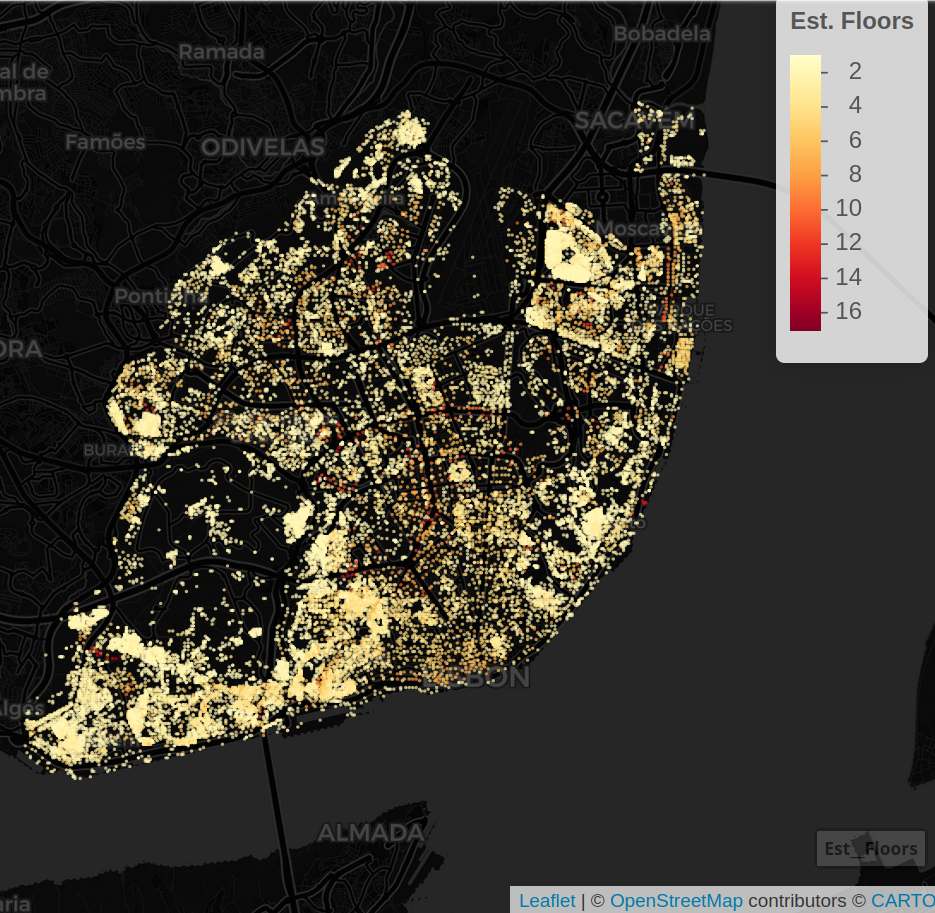
\includegraphics[keepaspectratio]{../images/Screenshot_20260217_172324.png}}

}

\caption{Lisbon buildings's estimated number of floors (mean: 2.94)}

\end{figure}%

\begin{figure}[H]

{\centering 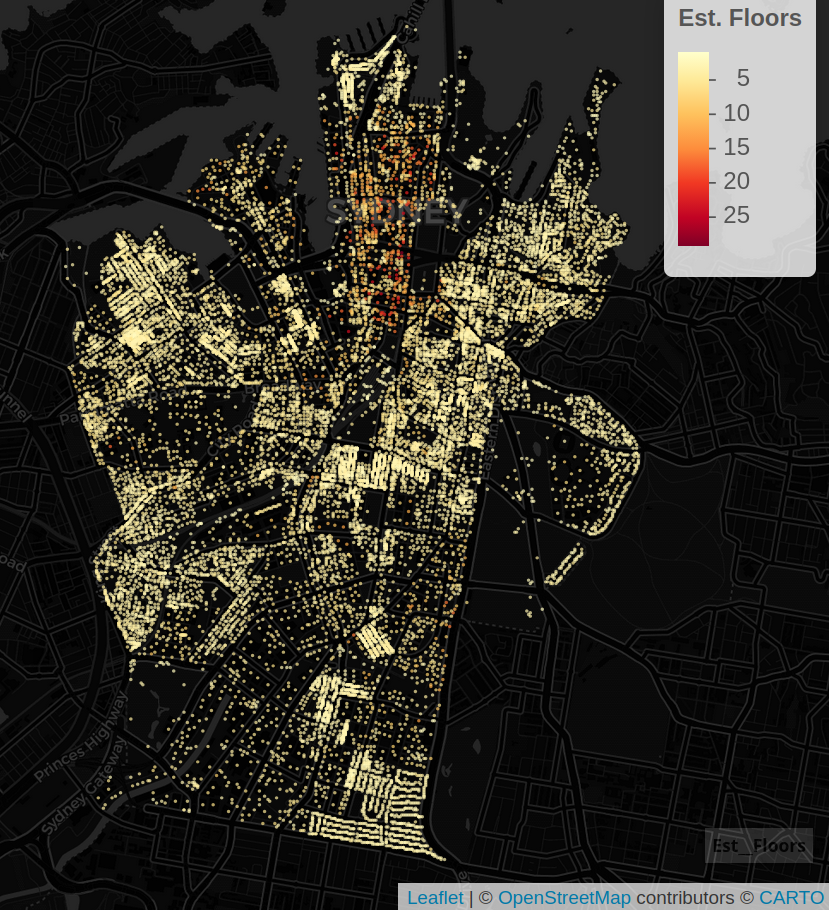
\includegraphics[width=4.6875in,height=\textheight,keepaspectratio]{../images/Screenshot_20260217_173136.png}

}

\caption{Sydney buildings's estimated number of floors (mean: 3.21)}

\end{figure}%

\begin{figure}[H]

{\centering 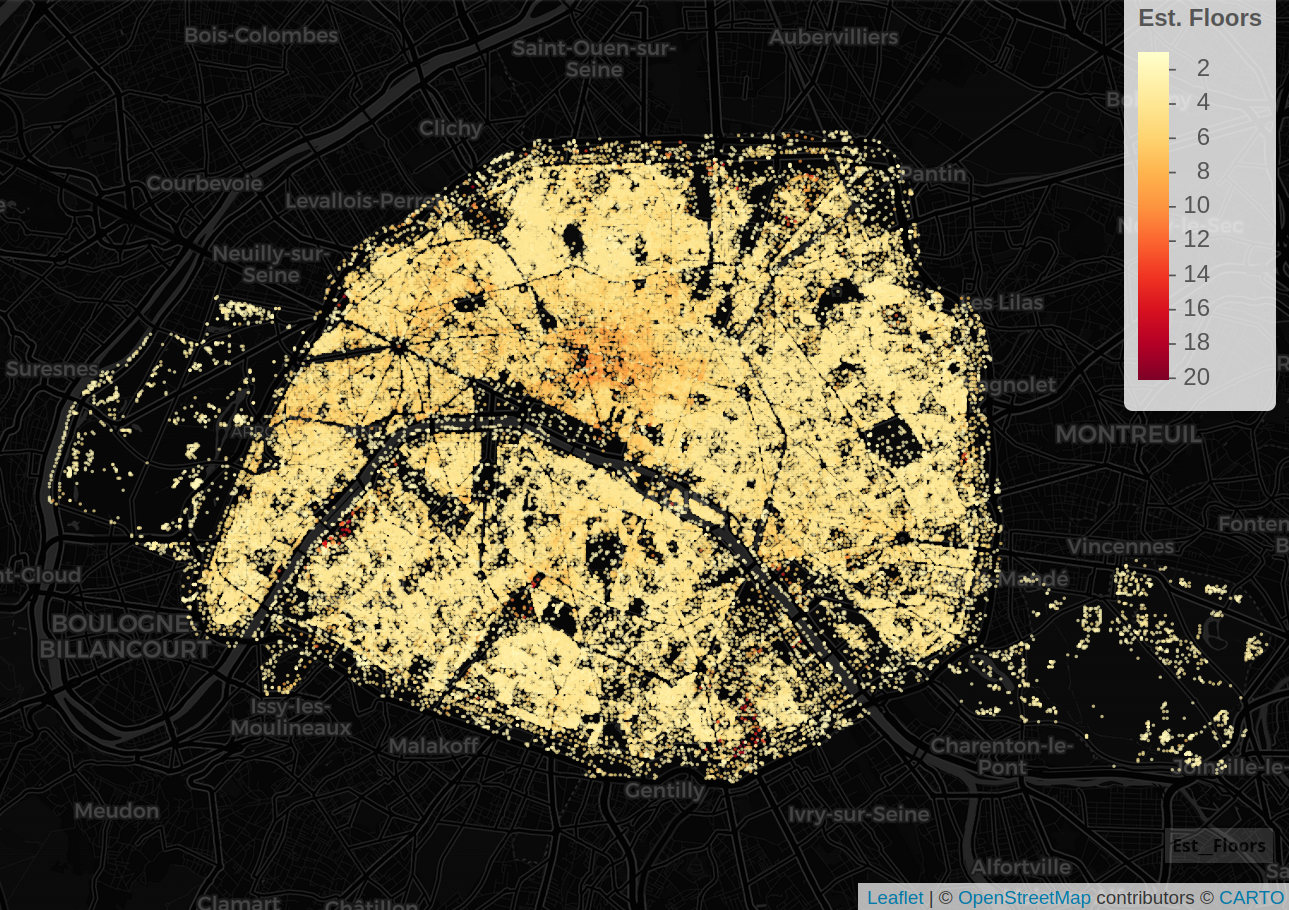
\includegraphics[width=4.6875in,height=\textheight,keepaspectratio]{../images/Screenshot_20260217_172645.png}

}

\caption{Paris buildings's estimated number of floors (mean: 3.92)}

\end{figure}%

Our trip distance distribution does not sound like a typical urban
bicycle trip distance distribution, with most bicycle trips raging from
2 to 5 km. Nevertheless, for the purpose of the study, to address
cycling infrastructure improvements, this may represent a minor
(although not irrelevant) issue.

\begin{figure}[H]

{\centering \pandocbounded{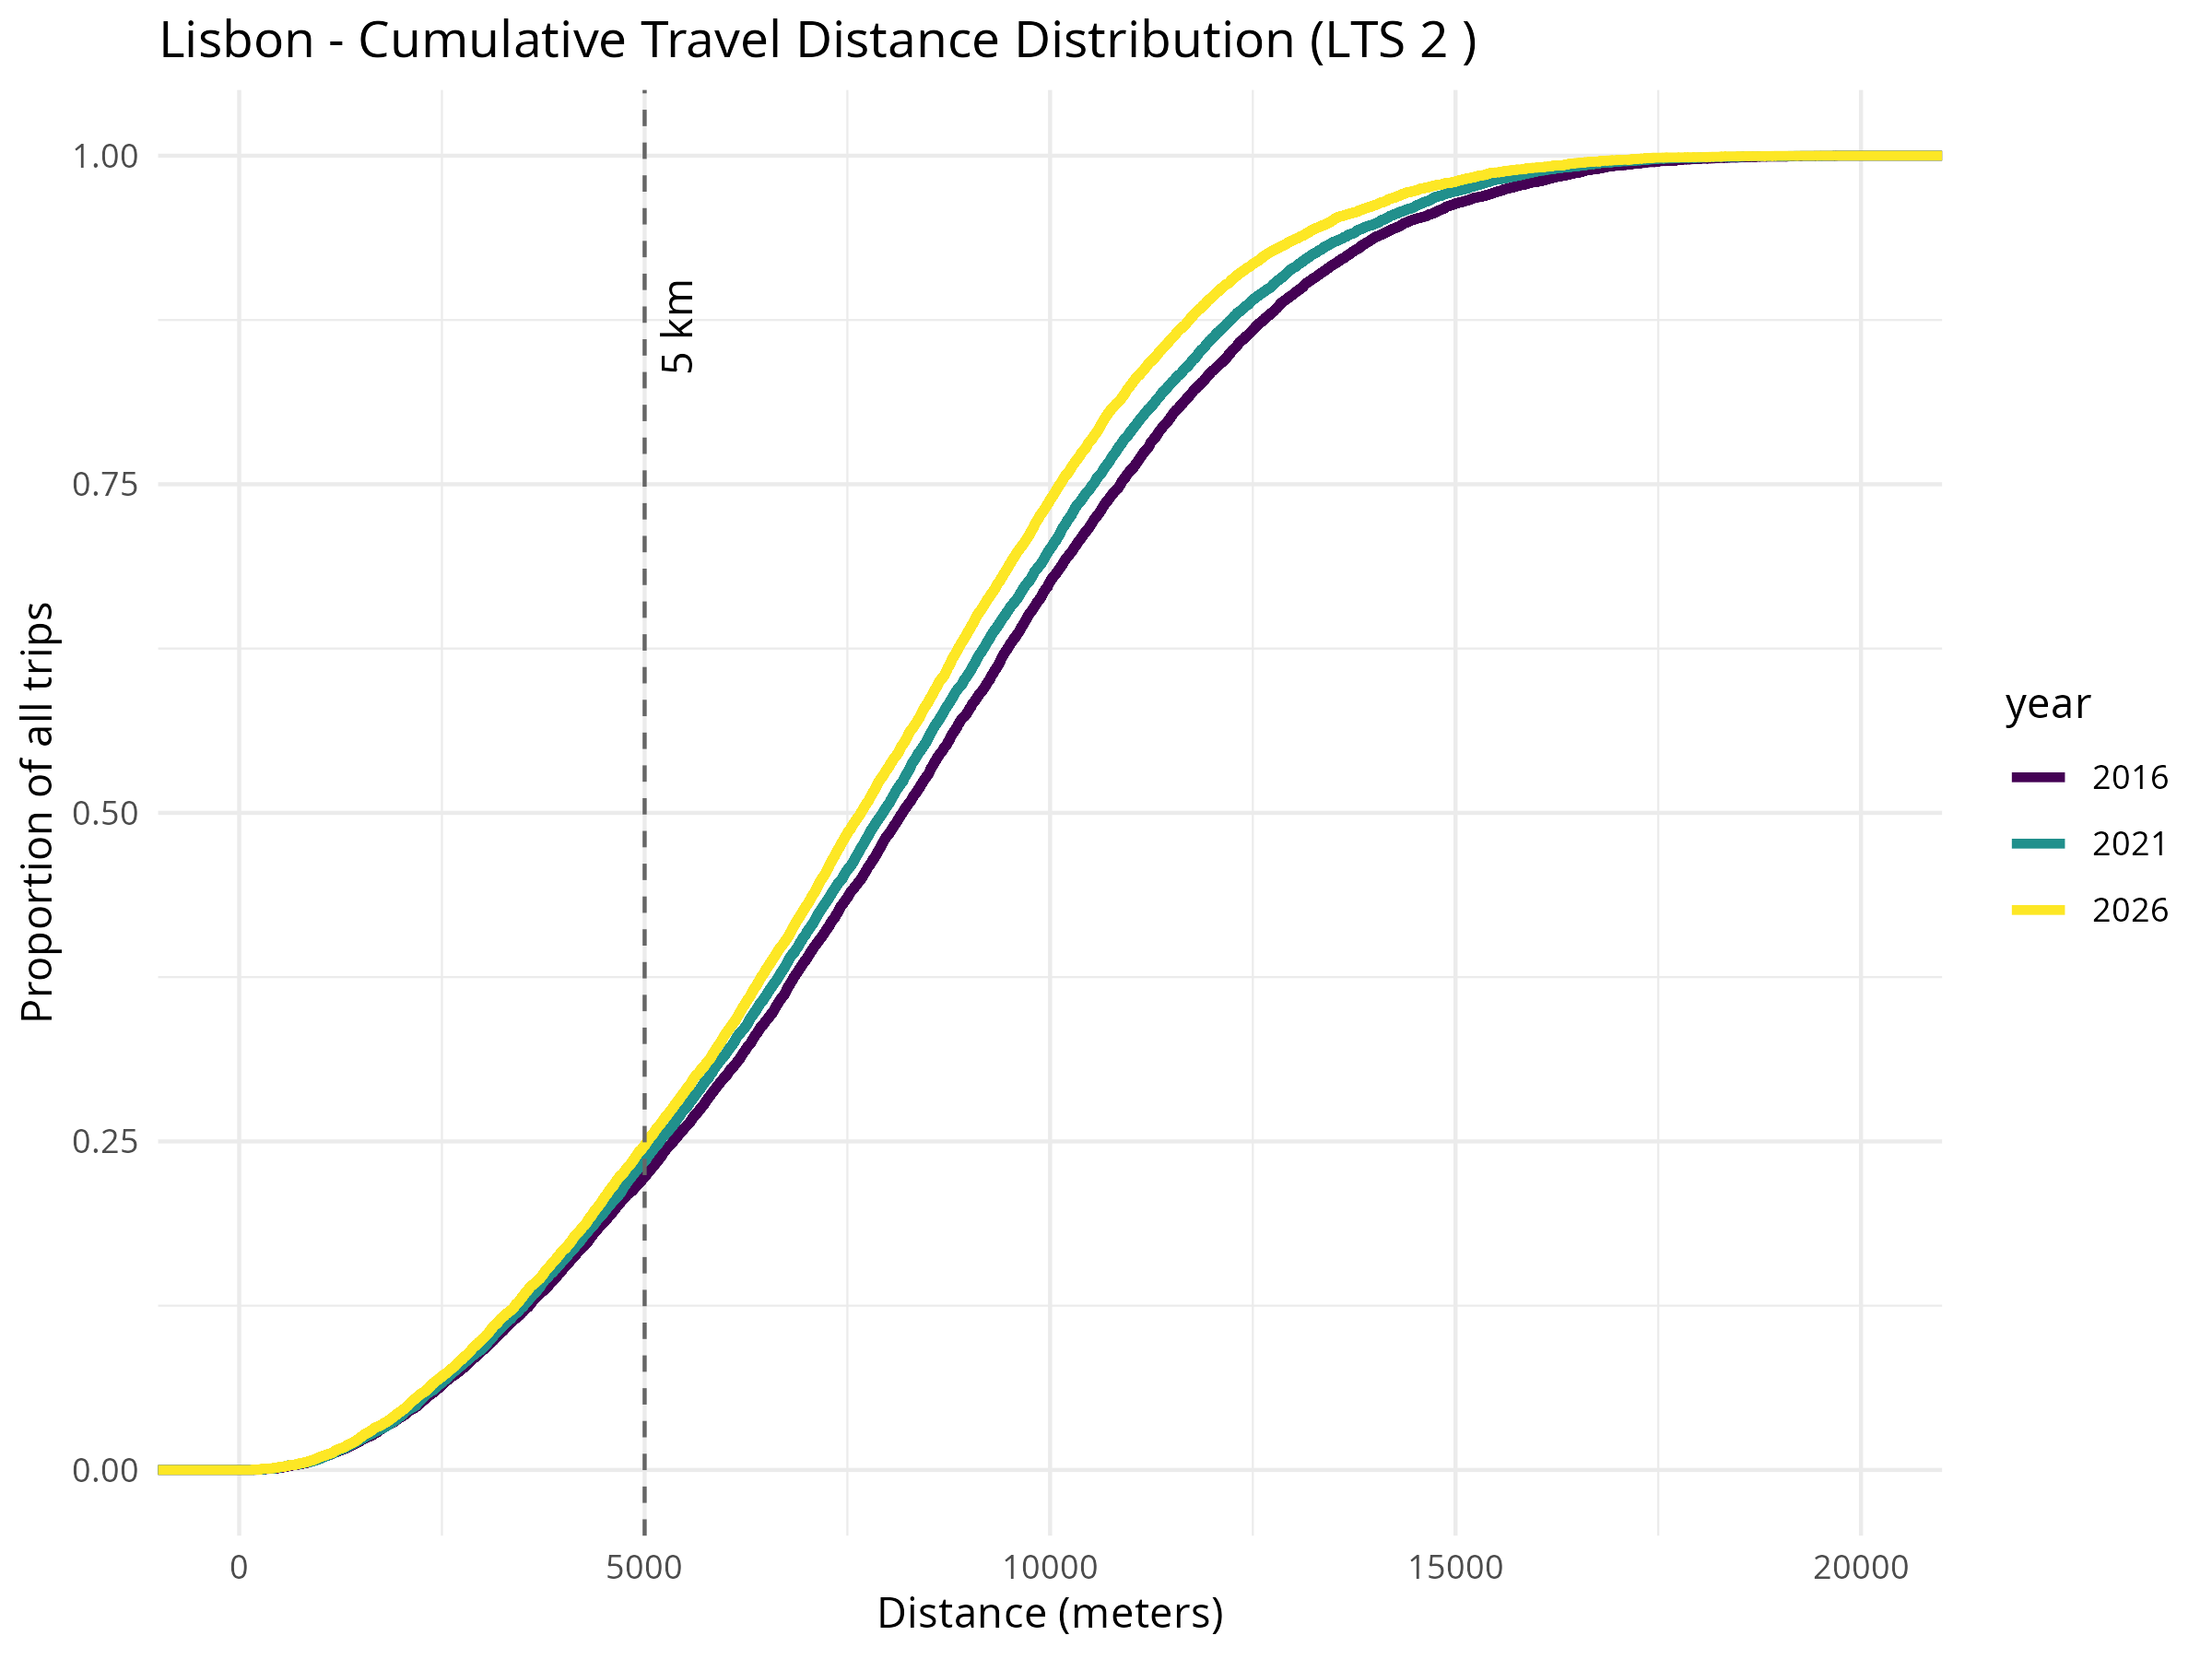
\includegraphics[keepaspectratio]{../data/pipeline/lisbon/results/cumulative_distance_lts2.png}}

}

\caption{Commulative distance distribution (Lisbon, LTS2). 75\% of the
trips are over 5km.}

\end{figure}%

Further developments of this research include the use a common
trip-length distribution in urban environments, such as distributions
described by Kou and Cai (2019), when analysing bike sharing data from 7
cities in the US, with the set parameters for commuting trips (in
miles).

\subsection{Routing}\label{routing}

We use r5r R package (Pereira et al. 2021) for routing in bicycle mode.
The parameters used are defined below:

\subsubsection{LTS}\label{lts}

LTS is defined by
\href{https://transweb.sjsu.edu/research/Low-Stress-Bicycling-and-Network-Connectivity}{Mineta
Transportation Institute} and us used in R5 as a set of ``surrogate
LTS'' rules to create similar classifications to the original
methodology that can be used with OSM data (Conway 2015) and
\url{https://docs.conveyal.com/learn-more/traffic-stress\#:~:text=Unsignalized\%20intersection\%20adjustment\%20round,entering\%20or\%20exiting\%20the\%20vertex.}
For each OSM edge:

\begin{verbatim}
    If way does not allow cars, assign LTS 1
    If way has highway=service tag, do not assign LTS in this round
    If way has a highway=residential or highway=living_street tag, assign LTS 1
    If tagged maxspeed value is less than 25 mph (40.25 km/h) and the number of lanes is less than 4 or unspecified, assign LTS 2
    If way has tag highway=unclassified, highway=tertiary, or highway=tertiary-link and the number of lanes is less than 4 or there is cycleway tag for the correct direction, assign LTS 2
    Otherwise, if there is a cycleway tag for the correct direction, assign LTS 3
    Otherwise, assign LTS 4
\end{verbatim}

In \texttt{R5} the cycling routing algorithm expects a \texttt{max\_lts}
(1, 2, 3, or 4). The R5 engine identifies all edges in OSM with a value
higher than \texttt{max\_lts}. For the edges exceeding the
\texttt{max\_lts}, the routing engine applies a time-cost of walking
speed (default 3.6 km/h), instead of cycling speed (default 12 km/h in
\texttt{r5r}), as if the cyclist would dismount and walk with the bike
on that segment (not accounting for mounting and dismounting time),
penalizing cost (time) in 3 times. So:

\begin{itemize}
\tightlist
\item
  If \texttt{edge.lts\ \textless{}=\ max\_lts} →
  \texttt{time\ =\ distance\ /\ bikeSpeed}.
\item
  If \texttt{edge.lts\ \textgreater{}\ max\_lts} →
  \texttt{time\ =\ distance\ /\ walkSpeed}.
\end{itemize}

Setting a low \texttt{max\_lts} (1 or 2) will result in routes that
favour separated bike paths and quiet backstreets. If no low-stress path
exists R5 provides a route with longer travel time, due to walk speed
penalty.

\subsubsection{Overline}\label{overline}

We use \texttt{stplanr} to overline the routes (Lovelace and Ellison
2018). This provides a better idea of which segments are used more in
routing routing, for each year and LTS levels.

The example in Sydney shows that\ldots{}

\begin{center}
\pandocbounded{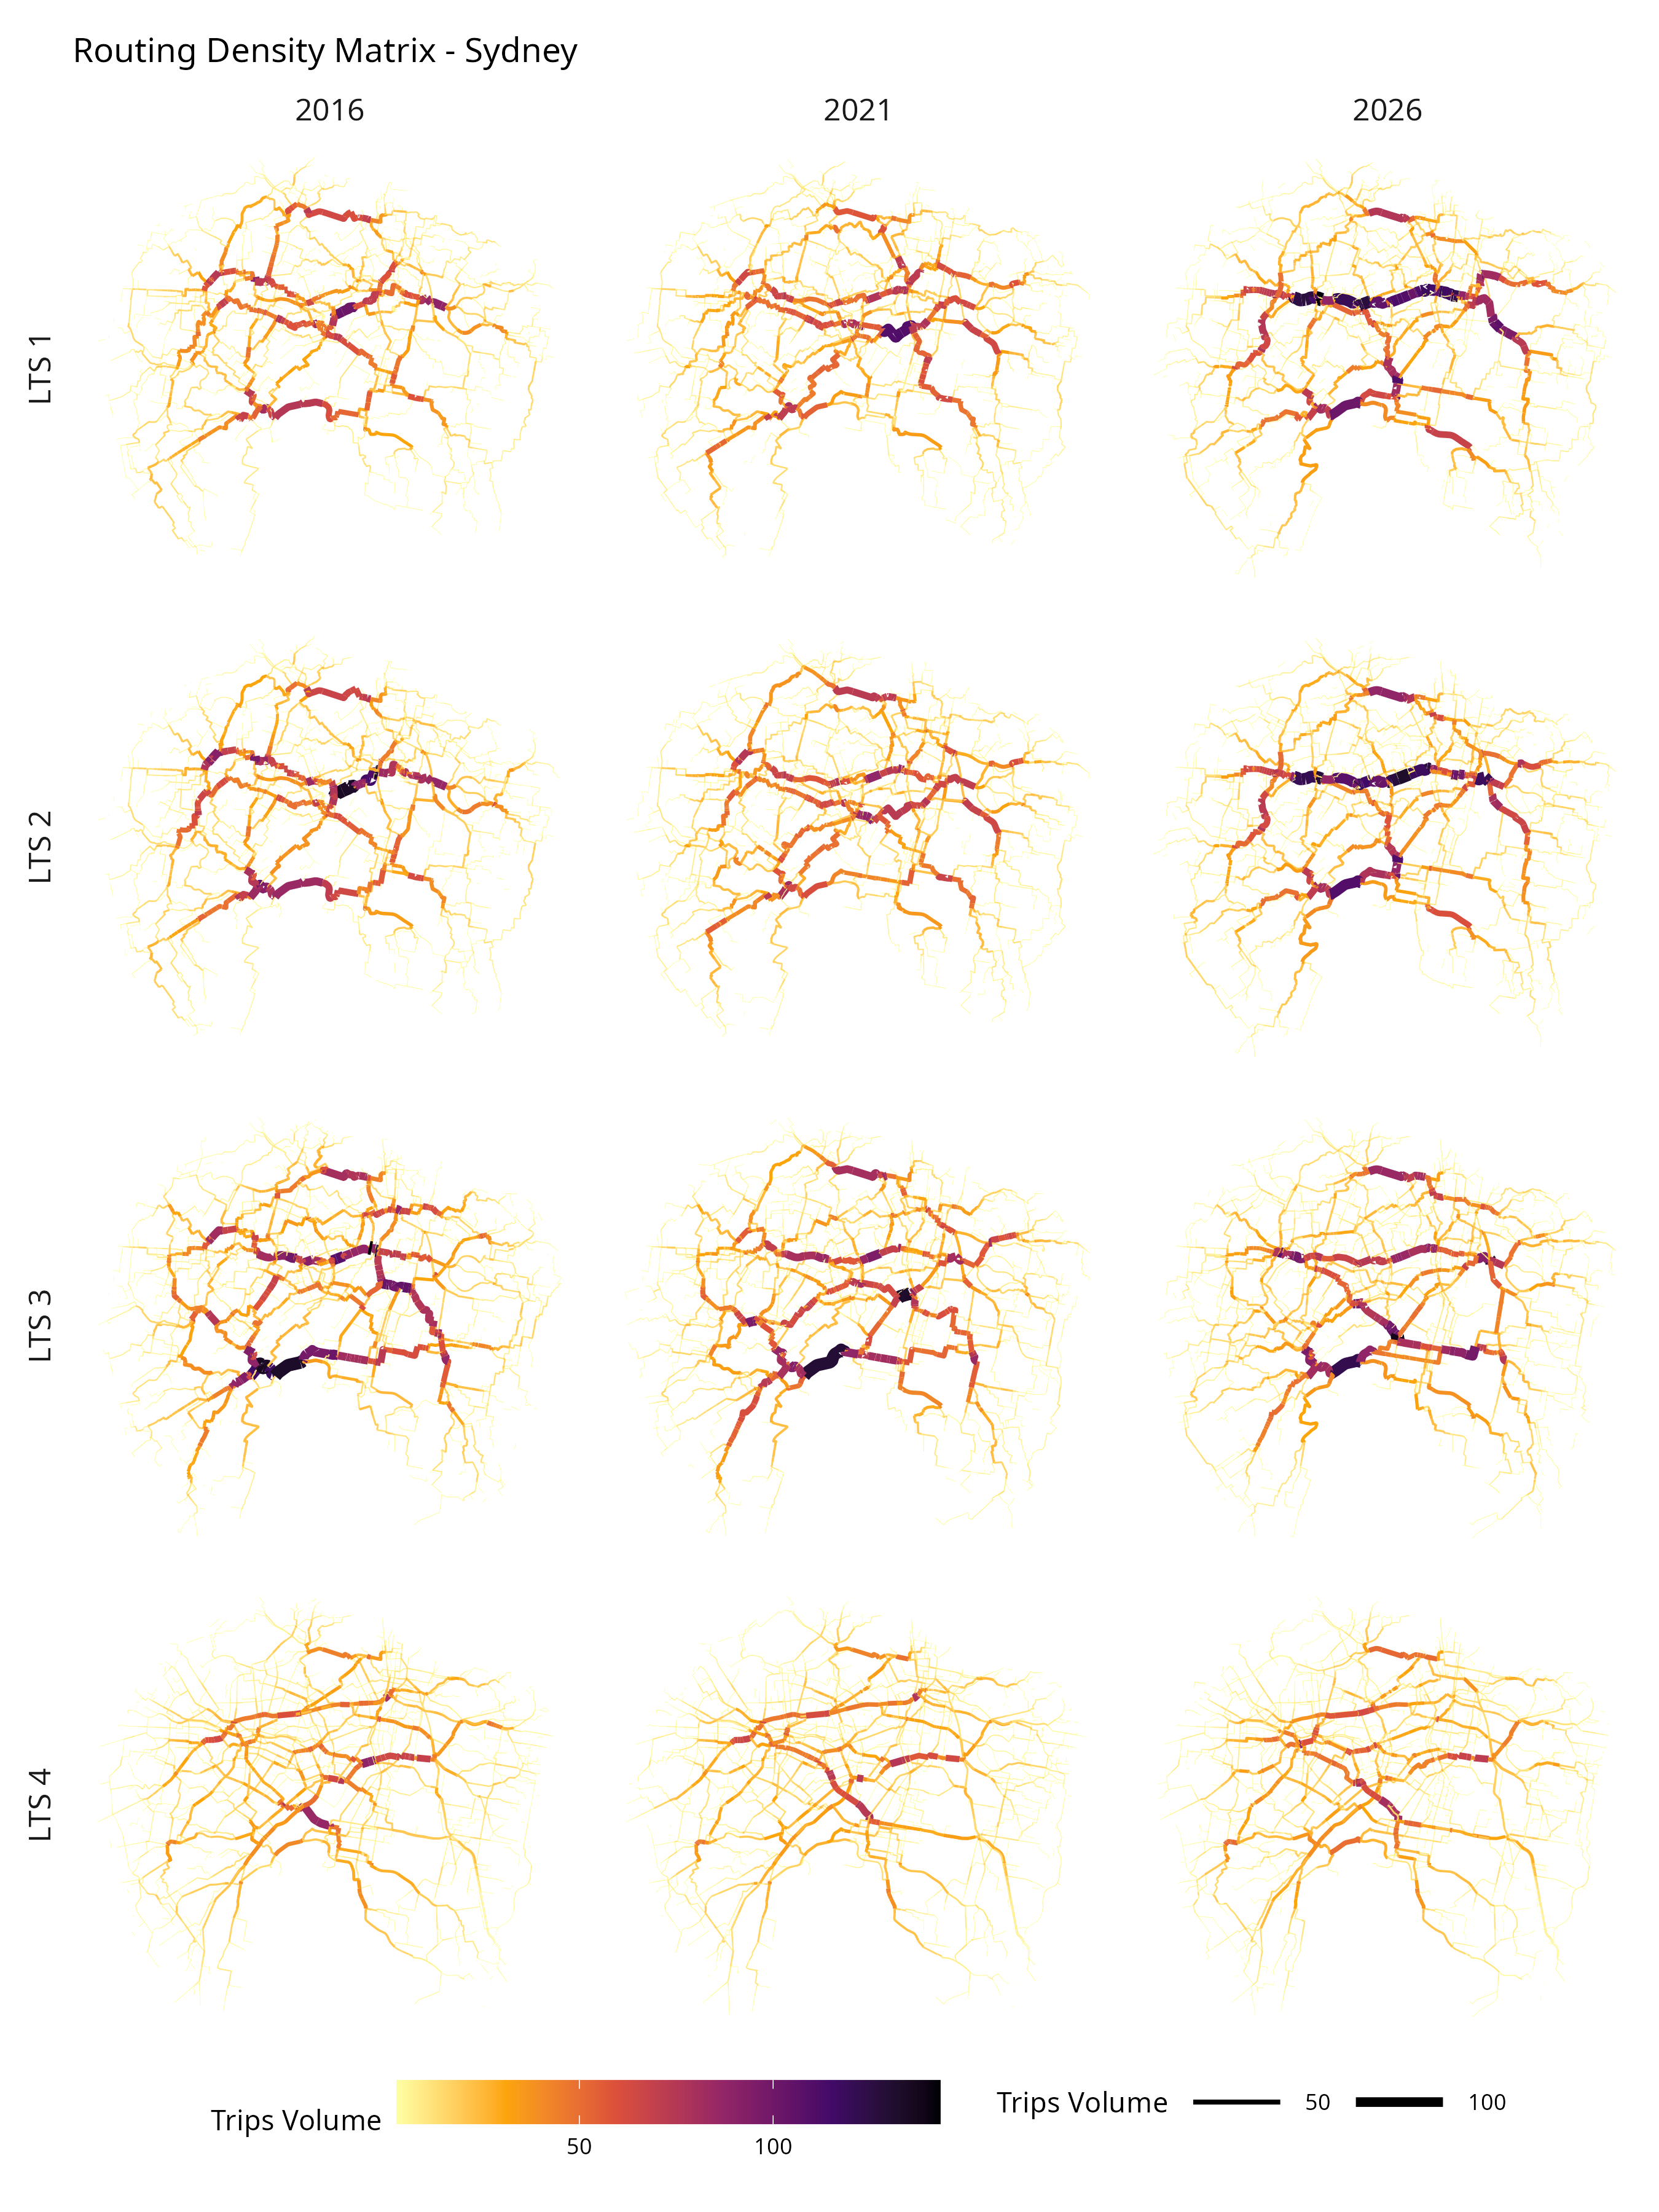
\includegraphics[keepaspectratio]{../data/pipeline/sydney/results/overline_matrix_test.png}}
\end{center}

Each city took, on average, \textbf{22 minutes} to process data, in a i9
32 core computer with 128 GB RAM,

\subsection{Code availability}\label{code-availability}

Code used to generate results from this study are available at
\href{https://temospena.github.com/Sydney/code/pipeline}{temospena.github.com/Sydney}.

\section{References}\label{references}

\phantomsection\label{refs}
\begin{CSLReferences}{1}{0}
\bibitem[\citeproctext]{ref-bernhoft2008}
Bernhoft, Inger Marie, and Gitte Carstensen. 2008. {``Preferences and
Behaviour of Pedestrians and Cyclists by Age and Gender.''}
\emph{Transportation Research Part F: Traffic Psychology and Behaviour}
11 (2): 83--95. \url{https://doi.org/10.1016/j.trf.2007.08.004}.

\bibitem[\citeproctext]{ref-boeing2017}
Boeing, Geoff. 2017. {``OSMnx: New Methods for Acquiring, Constructing,
Analyzing, and Visualizing Complex Street Networks.''} \emph{Computers,
Environment and Urban Systems} 65 (September): 126--39.
\url{https://doi.org/10.1016/j.compenvurbsys.2017.05.004}.

\bibitem[\citeproctext]{ref-cambra2019a}
Cambra, Paulo Jorge, Alexandre Gonçalves, and Filipe Moura. 2019. {``The
Digital Pedestrian Network in Complex Urban Contexts: A Primer
Discussion on Typological Specifications.''} \emph{Finisterra}, May,
155--170 Pages. \url{https://doi.org/10.18055/FINIS16414}.

\bibitem[\citeproctext]{ref-cambra2019}
Cambra, Paulo, and Filipe Moura. 2020. {``How Does Walkability Change
Relate to Walking Behavior Change? Effects of a Street Improvement in
Pedestrian Volumes and Walking Experience.''} \emph{Journal of Transport
and Health} 16 (November 2019): 100797--97.
\url{https://doi.org/10.1016/j.jth.2019.100797}.

\bibitem[\citeproctext]{ref-christ2023}
Christ, Ana Karina, Miguel Costa, Manuel Marques, Carlos Roque, and
Filipe Moura. 2023. {``Perceiving Objective Cycling Safety: A Systematic
Literature Review.''} In, 72:1380--87.
\url{https://doi.org/10.1016/j.trpro.2023.11.601}.

\bibitem[\citeproctext]{ref-conway2015}
Conway, Mathew. 2015. {``Better Measures of Bike Accessibility.''}
\url{https://medium.com/conveyal-blog/better-measures-of-bike-accessibility-d875ae5ed831}.

\bibitem[\citeproctext]{ref-cooper2015}
Cooper, Crispin H. V. 2015. {``Spatial Localization of Closeness and
Betweenness Measures: A Self-Contradictory but Useful Form of Network
Analysis.''} \emph{International Journal of Geographical Information
Science} 29 (8): 1293--1309.
\url{https://doi.org/10.1080/13658816.2015.1018834}.

\bibitem[\citeproctext]{ref-cooper2020}
Cooper, Crispin H. V., and Alain J. F. Chiaradia. 2020. {``sDNA: 3-d
Spatial Network Analysis for GIS, CAD, Command Line \& Python.''}
\emph{SoftwareX} 12 (July): 100525.
\url{https://doi.org/10.1016/j.softx.2020.100525}.

\bibitem[\citeproctext]{ref-costa2021}
Costa, Miguel, Manuel Marques, and Filipe Moura. 2021. {``A Circuity
Temporal Analysis of Urban Street Networks Using Open Data: A Lisbon
Case Study.''} \emph{ISPRS International Journal of Geo-Information} 10
(7): 453. \url{https://doi.org/10/gmf8c9}.

\bibitem[\citeproctext]{ref-fuxe9lix2020}
Félix, Rosa, Paulo Cambra, and Filipe Moura. 2020. {``Build It and Give
{`}Em Bikes, and They Will Come: The Effects of Cycling Infrastructure
and Bike-Sharing System in Lisbon.''} \emph{Case Studies on Transport
Policy} 8 (2): 672--82.
\url{https://doi.org/10.1016/j.cstp.2020.03.002}.

\bibitem[\citeproctext]{ref-fuxe9lix2022}
Félix, Rosa, Robin Lovelace, and Filipe Moura. 2022. {``biclaR:
Ferramenta de Apoio Ao Planeamento Da Rede Ciclável Na Área
Metropolitana de Lisboa.''} Lisboa.
\url{https://biclar.tmlmobilidade.pt}.

\bibitem[\citeproctext]{ref-fuxe9lix2019}
Félix, Rosa, Filipe Moura, and Kelly J Clifton. 2019. {``Maturing Urban
Cycling: Comparing Barriers and Motivators to Bicycle of Cyclists and
Non-Cyclists in Lisbon, Portugal.''} \emph{Journal of Transport \&
Health} 15: 100628--28. \url{https://doi.org/10.1016/j.jth.2019.100628}.

\bibitem[\citeproctext]{ref-fuxe9lix2025}
Félix, Rosa, Filipe Moura, and Kelly J. Clifton. 2025. {``The Hierarchy
of Cycling Needs: Modeling the Self-Assessed Propensity to Bicycle.''}
\emph{Journal of Urban Mobility} 7 (June): 100130.
\url{https://doi.org/10.1016/j.urbmob.2025.100130}.

\bibitem[\citeproctext]{ref-fernandes2020}
Fernandes, P., C. Sousa, J. Macedo, and M. C. Coelho. 2020. {``How to
Evaluate the Extent of Mobility Strategies in a University Campus: An
Integrated Analysis of Impacts.''} \emph{International Journal of
Sustainable Transportation} 14 (2): 120--36.
\url{https://doi.org/10.1080/15568318.2018.1531183}.

\bibitem[\citeproctext]{ref-furth2016}
Furth, Peter G., Maaza C. Mekuria, and Hilary Nixon. 2016. {``Network
Connectivity for Low-Stress Bicycling.''} \emph{Transportation Research
Record: Journal of the Transportation Research Board} 2587 (1): 41--49.
\url{https://doi.org/10.3141/2587-06}.

\bibitem[\citeproctext]{ref-gehrke2020}
Gehrke, Steven R., Armin Akhavan, Peter G. Furth, Qi Wang, and Timothy
G. Reardon. 2020. {``A Cycling-Focused Accessibility Tool to Support
Regional Bike Network Connectivity.''} \emph{Transportation Research
Part D: Transport and Environment} 85 (August): 102388.
\url{https://doi.org/10.1016/j.trd.2020.102388}.

\bibitem[\citeproctext]{ref-giacomin2015}
Giacomin, David J, and David M Levinson. 2015. {``Road Network Circuity
in Metropolitan Areas.''} \emph{Environment and Planning B: Planning and
Design} 42 (6): 1040--53. \url{https://doi.org/10.1068/b130131p}.

\bibitem[\citeproctext]{ref-heinen2010}
Heinen, Eva, Bert van Wee, and Kees Maat. 2010. {``Commuting by Bicycle:
An Overview of the Literature.''} \emph{Transport Reviews} 30 (1):
59--96. \url{https://doi.org/10.1080/01441640903187001}.

\bibitem[\citeproctext]{ref-humberto2023}
Humberto, Mateus, Rosa Félix, and Filipe Moura. 2023. {``How Equal Is
Accessibility to Cycling Infrastructure? A Ranking to Compare
Territories in Lisbon, Portugal.''} In, 72:2472--78.
\url{https://doi.org/10.1016/j.trpro.2023.11.752}.

\bibitem[\citeproctext]{ref-kou2019}
Kou, Zhaoyu, and Hua Cai. 2019. {``Understanding Bike Sharing Travel
Patterns: An Analysis of Trip Data from Eight Cities.''} \emph{Physica
A: Statistical Mechanics and Its Applications} 515 (February): 785--97.
\url{https://doi.org/10.1016/j.physa.2018.09.123}.

\bibitem[\citeproctext]{ref-levinson2012}
Levinson, David. 2012. {``Network Structure and City Size.''} Edited by
Yamir Moreno. \emph{PLoS ONE} 7 (1): e29721.
\url{https://doi.org/10.1371/journal.pone.0029721}.

\bibitem[\citeproctext]{ref-lovelace2018}
Lovelace, Robin, and Richard Ellison. 2018. {``Stplanr: A Package for
Transport Planning.''} \emph{The R Journal} 10 (2): 7--23.
\url{https://doi.org/10/gkb499}.

\bibitem[\citeproctext]{ref-lovelace2022}
Lovelace, Robin, Rosa Félix, and Dustin Carlino. 2022. {``Jittering: A
Computationally Efficient Method for Generating Realistic Route Networks
from Origin-Destination Data.''} \emph{Findings}, April, 33873.
\url{https://doi.org/10.32866/001c.33873}.

\bibitem[\citeproctext]{ref-lovelace2017}
Lovelace, Robin, Anna Goodman, Rachel Aldred, and James Woodcock. 2017.
{``The Propensity to Cycle Tool: An Open Source Online System for
Sustainable Transport Planning Developer.''} \emph{Journal of Transport
and Land Use} 10 (1): 505--28.
\url{https://doi.org/10.5198/jtlu.2016.862}.

\bibitem[\citeproctext]{ref-lovelace2024}
Lovelace, Robin, Joey Talbot, Eugeni Vidal-Tortosa, Hussein Mahfouz,
Elaine Brick, Peter Wright, Gary O'Toole, Dan Brennan, and Suzanne
Meade. 2024. {``Cycle Route Uptake and Scenario Estimation (CRUSE): An
Approach for Developing Strategic Cycle Network Planning Tools.''}
\emph{European Transport Research Review} 16 (1): 55.
\url{https://doi.org/10.1186/s12544-024-00668-8}.

\bibitem[\citeproctext]{ref-macedo2017}
Macedo, Joaquim, Fernanda Rodrigues, and Fernando Tavares. 2017.
{``Urban Sustainability Mobility Assessment: Indicators Proposal.''}
\emph{Energy Procedia} 134 (October): 731--40.
\url{https://doi.org/10.1016/j.egypro.2017.09.569}.

\bibitem[\citeproctext]{ref-matos2021}
Matos, Francisco Lé De, José Maria Fernandes, Carlos Sampaio, Joaquim
Macedo, Margarida C. Coelho, and Jorge Bandeira. 2021. {``Development of
an Information System for Cycling Navigation.''} \emph{Transportation
Research Procedia} 52: 107--14.
\url{https://doi.org/10.1016/j.trpro.2021.01.012}.

\bibitem[\citeproctext]{ref-moura2017}
Moura, Filipe, Joana Magalhães, and Luis Picado Santos. 2017. {``Growing
from Incipient to Potentially Large Cycle Networks: Screening the Road
Network of the Consolidated Urban Area of Lisbon.''} \emph{European
Journal of Transport and Infrastructure Research} 17 (1): 170--90.

\bibitem[\citeproctext]{ref-murphy2019}
Murphy, Brendan, and Andrew Owen. 2019. {``Implementing Low-Stress
Bicycle Routing in National Accessibility Evaluation.''}
\emph{Transportation Research Record: Journal of the Transportation
Research Board} 2673 (5): 240--49.
\url{https://doi.org/10.1177/0361198119837179}.

\bibitem[\citeproctext]{ref-niaki2025}
Niaki, Matin S. Nabavi, Jean-Simon Bourdeau, Luis Miranda-Moreno, and
Nicolas Saunier. 2025. {``Cycling Network Discontinuities as Indicators
for Performance Evaluation: Case Study in Four Cities.''}
\emph{Transportation Research Procedia} 82: 1071--88.
\url{https://doi.org/10.1016/j.trpro.2024.12.114}.

\bibitem[\citeproctext]{ref-pereira2021}
Pereira, Rafael H. M., Marcus Saraiva, Daniel Herszenhut, Carlos Kaue
Vieira Braga, and Matthew Wigginton Conway. 2021. {``R5r: Rapid
Realistic Routing on Multimodal Transport Networks with
R{\textsuperscript{5}} in R.''} \emph{Findings}, March, 21262.
\url{https://doi.org/10.32866/001c.21262}.

\bibitem[\citeproctext]{ref-reggiani2022}
Reggiani, Giulia, Tim Van Oijen, Homayoun Hamedmoghadam, Winnie Daamen,
Hai L. Vu, and Serge Hoogendoorn. 2022. {``Understanding Bikeability: A
Methodology to Assess Urban Networks.''} \emph{Transportation} 49 (3):
897--925. \url{https://doi.org/10.1007/s11116-021-10198-0}.

\bibitem[\citeproctext]{ref-rissel2015}
Rissel, Chris, Stephen Greaves, Li Ming Wen, Melanie Crane, and Chris
Standen. 2015. {``Use of and Short-Term Impacts of New Cycling
Infrastructure in Inner-Sydney, Australia: A Quasi-Experimental
Design.''} \emph{International Journal of Behavioral Nutrition and
Physical Activity} 12 (1): 129.
\url{https://doi.org/10.1186/s12966-015-0294-1}.

\bibitem[\citeproctext]{ref-schon2024}
Schön, Peter, Eva Heinen, and Bendik Manum. 2024. {``A Scoping Review on
Cycling Network Connectivity and Its Effects on Cycling.''}
\emph{Transport Reviews} 44 (4): 912--36.
\url{https://doi.org/10.1080/01441647.2024.2337880}.

\bibitem[\citeproctext]{ref-schon2026}
---------. 2026. {``Route-Based Network Analysis: {``}Route
Betweenness{''} and {``}Route Link Density{''} Applied to a Study of a
Proposed Bridge in Trondheim.''} \emph{Journal of Transport Geography}
130 (January): 104491.
\url{https://doi.org/10.1016/j.jtrangeo.2025.104491}.

\bibitem[\citeproctext]{ref-schoner2014}
Schoner, Jessica E., and David M. Levinson. 2014. {``The Missing Link:
Bicycle Infrastructure Networks and Ridership in 74 US Cities.''}
\emph{Transportation} 41 (6): 1187--1204.
\url{https://doi.org/10.1007/s11116-014-9538-1}.

\bibitem[\citeproctext]{ref-szell2021}
Szell, Michael, Sayat Mimar, Tyler Perlman, Gourab Ghoshal, and Roberta
Sinatra. 2021. {``Growing Urban Bicycle Networks.''}
\emph{arXiv:2107.02185 {[}Physics{]}}, July.
\url{http://arxiv.org/abs/2107.02185}.

\bibitem[\citeproctext]{ref-tera2025}
Tera, H., A. Hadachi, and M. Pourmoradnasseri. 2025. {``Data-Driven
Approach for Assessing the Impact of Newly Developed Cycling
Infrastructure on Cyclists' Route Choice.''} \emph{Journal of Transport
Geography} 123 (February): 104094.
\url{https://doi.org/10.1016/j.jtrangeo.2024.104094}.

\bibitem[\citeproctext]{ref-vale2016}
Vale, David S, and Mauro Pereira. 2016. {``Influence on Pedestrian
Commuting Behavior of the Built Environment Surrounding Destinations: A
Structural Equations Modeling Approach.''} \emph{International Journal
of Sustainable Transportation} 10 (8): 730--41.
\url{https://doi.org/10.1080/15568318.2016.1144836}.

\bibitem[\citeproctext]{ref-vandermeer2024}
Van Der Meer, Lucas, Christian Werner, and Martin Loidl. 2024.
{``Assessment of Bicycle Accessibility to Mobility Hubs Under Different
Criteria for Cycling Network Quality.''} \emph{AGILE: GIScience Series}
5 (May): 1--7. \url{https://doi.org/10.5194/agile-giss-5-48-2024}.

\bibitem[\citeproctext]{ref-wang2026}
Wang, Zhao, Hang Hu, Hussein Mahfouz, Juan Pablo Fonseca-Zamora, Martin
Lucas-Smith, Dustin Carlino, Angus Calder, et al. 2026. {``Corenet: A
Flexible Framework for Generating and Prioritising Core Cycle Network
Designs.''} \emph{Journal of Transport Geography} 131 (February):
104549. \url{https://doi.org/10.1016/j.jtrangeo.2026.104549}.

\bibitem[\citeproctext]{ref-weikl2023}
Weikl, Simone, and Patricia Mayer. 2023. {``Data-Driven Quality
Assessment of Cycling Networks.''} \emph{Frontiers in Future
Transportation} 4 (March): 1127742.
\url{https://doi.org/10.3389/ffutr.2023.1127742}.

\bibitem[\citeproctext]{ref-werner2024}
Werner, Christian, Lucas Van Der Meer, Dana Kaziyeva, Petra Stutz, Robin
Wendel, and Martin Loidl. 2024. {``Bikeability of Road Segments: An
Open, Adjustable and Extendible Model.''} \emph{Journal of Cycling and
Micromobility Research} 2 (December): 100040.
\url{https://doi.org/10.1016/j.jcmr.2024.100040}.

\bibitem[\citeproctext]{ref-xie2007}
Xie, Feng, and David Levinson. 2007. {``Measuring the Structure of Road
Networks.''} \emph{Geographical Analysis} 39 (3): 336--56.
\url{https://doi.org/10.1111/j.1538-4632.2007.00707.x}.

\bibitem[\citeproctext]{ref-xing2025}
Xing, Ruru, ZePeng Yang, Xinghua Zhang, Yiwen Liang, Tao Yang, and Fei
Wang. 2025. {``Identifying Strong Connectivity in Urban Road Networks
Considering Traffic Constraints: An Analysis of Road Networks With
Different Patterns.''} Edited by Indrajit Ghosh. \emph{Journal of
Advanced Transportation} 2025 (1): 3589423.
\url{https://doi.org/10.1155/atr/3589423}.

\bibitem[\citeproctext]{ref-zhu2025}
Zhu, Xiao Xiang, Sining Chen, Fahong Zhang, Yilei Shi, and Yuanyuan
Wang. 2025. {``GlobalBuildingAtlas: An Open Global and Complete Dataset
of Building Polygons, Heights and LoD1 3D Models.''} \emph{Earth System
Science Data} 17 (12): 6647--68.
\url{https://doi.org/10.5194/essd-17-6647-2025}.

\end{CSLReferences}

\section{Acknowledgements}\label{acknowledgements}




\end{document}
